\documentclass[10pt]{reportMaster}

\title{Recommender system for multiple online shops}
\author{S.\ Deckers}
\id{DKE 17-04}
\department{Artificial Intelligence}
\committee{Dr. K. Driessens \\ Dr. E.N. Smirnov}
\date{25th January 2017}


% new line instead of indent for new paragraph
\usepackage[parfill]{parskip}
\usepackage{dsfont}
\usepackage{amsmath}
\usepackage{textcomp} % for texttimes
\usepackage{algpseudocode}
\usepackage{algorithm}

% figure stuff
\usepackage{graphicx}
\usepackage{caption}
\usepackage{subcaption}

\usepackage{url}


\begin{document}
\maketitle

\tableofcontents

\listoffigures
\listoftables
\listofalgorithms

%==============================================================
\chapter{Introduction}
Recommendation systems are systems that aim to make personalized recommendations to its users.
They are widely used in the world wide web in different contexts such as movie recommendation in the streaming service Netflix or music recommendation as in last.fm as well as in e-commerce to recommend products, that the user might purchase.
They seek to provide users with items that are new to them or they might not have discovered otherwise.

%Probelms with e-commerce data
While in the context of Netflix or last.fm the users actively search for new movies or music and intentionally use the recommendation system, in the context of e-commerce recommendations are usually shown while browsing the website.
This also reflects in the kind of input the users give to the recommendation system.
In systems like Netflix  \cite{netflixPrize} and last.fm \cite{implExplComparisonLastfm} the users give explicit feedback to different items in the form of ratings to express, how much a user likes an item, or by simply stating, whether the user likes or dislikes an item.
E-commerce services in contrast need to derive user preferences from their purchase or browsing behaviour.
This kind of feedback is called implicit feedback.
In \cite{implExplComparisonLastfm} a comparison of implicit and explicit feedback data in the context of music recommendation is given, showing that they perform similarly.
Though in e-commerce this kind of feedback leads to problems for several reasons.
First implicit feedback might be noisy, since it bases on the assumption that a user is interested in an item if he purchased it.
This assumption is not necessarily true, because he may have bought it for a friend or may be unsatisfied with the product.
If a user watches a movie, he is able to give it a low rating.
This option is not necessarily available within online shops.
Moreover implicit e-commerce datasets do not contain any information about negative feedback.
Positive feedback, i.e. interest in a product, can be derived from purchases, shopping cart entries or page visits, but there is no indication for disinterest in an item.
While in a rating dataset items that are not liked by the user have a low rating and not rated ones are considered unknown, in e-commerce datasets it is unknown, whether items, that have not been purchased, are not interesting or not known to the user.
This raises two problems.
It may happen, that a user gets repeatedly recommendations of the same items, he does not need, since he has no chance to mark them as uninteresting.
This might lead to decreased user satisfaction and recommendation performance, but this issue will not be addressed in the scope of this thesis.
The second problem is, that negative feedback is necessary for some recommendation models, since in general machine learning models cannot be trained on instances of one class only.
So some sampling techniques need to be investigated, to figure out how to treat unknown instances.

%Comparison of different techniques
There are different recommendation techniques, that will be compared within this thesis.
In general the performance of a specific recommendation technique depends on the data it is applied on.
Recommender systems have been applied to data from various domains like movies, songs, news articles, books or shops.
The data vary in size, sparseness, distribution, type of feedback and diversity of items.
For example while services like Netflix only provide movies, Amazon provides items from very different domains.
To find a suitable technique for e-commerce data, different techniques are implemented and compared to each other.

%Large sparse datasets
A general challenge for recommendation is the high dimensionality and sparseness of the data.
Usually there is a high amount of users and items, but a single user only interacts with a relatively small amount of items and many items are only considered by a small amount of users.
This must be taken into account for the choice of recommendation algorithms as well as for implementation aspects, especially for the representation of the large sparse matrix.

%todo could add that there are interactive systems or configarionable ones
%todo also could add different requirements/criteria from the handbook

\section{Research questions}
% Investigate different techniques, see how they perform, what are their pro and cons
\paragraph{Which types of recommendation algorithms are applicable to \\e-commerce data?}
The goal of this thesis is to find a recommendation system for e-commerce datasets.
It is required to provide accurate recommendations in terms of the mean average precision described in section \ref{sec:eval} as well fast recommendations to preserve user satisfaction when using the online shops.
So it is elaborated which types of recommendation algorithms are applicable to e-commerce.
The first task of this thesis is to implement different recommendation techniques, measure their performance on an e-commerce dataset and analyse their advantages and drawbacks.
The implemented techniques include different collaborative filtering approaches, i.e. memory-based and model-based collaborative filtering, and content-based recommendation, see section \ref{sec:recommenderSystems}.

% Implicit feedback problem
\paragraph{Can logistic regression improve performance of model-based collaborative filtering?}
Many known techniques, especially model-based collaborative filtering techniques, have been developed to perform well only on rating data sets.
They need to be adjusted to implicit feedback datasets, especially regarding the lack of negative feedback.
So a new collaborative filtering algorithm is developed, that learns latent factors from binary feedback by applying logistic regression.

\paragraph{Can AdaBoost enhance model-based collaborative filtering on \\e-commerce data?}
To overcome the problems of missing negative feedback and the skewed data distribution an AdaBoost approach is applied to the developed algorithm.
A single collaborative filtering model performs more updates of user and item features with more purchases, since more instances are available for training.
An AdaBoost approach should also emphasize training of user and items with fewer purchases to ensure a more balanced training of different user and item features. 

\paragraph{Can alternative prediction rules for AdaBoost improve prediction results?}
AdaBoost results in several models to compute recommendations for many users.
The performance of those model may vary for different users or item.
So prediction rules are developed, that take the prediction errors of users or items into account instead of the full model error as in traditional AdaBoost approaches.

% How do they correlate, maybe hybrid
\paragraph{May hybrid recommenders of the presented approaches be able to improve recommendation performance?}
In the last step of this thesis it will be investigated, whether hybrid recommendation approaches are able to improve precision.
The single recommendation systems are evaluated and their errors are compared in order to find a hybrid technique, that makes use of the benefits of different recommenders.
It was shown among others by \cite{hybridSurvey} or \cite{hybridcfcbClaypool} that some hybrid recommenders are able to outperform single recommenders.
\cite{hybridSurvey} offers a survey of different combinations of recommenders applied to a restaurant recommender systems.
In \cite{hybridcfcbClaypool} a weighted hybrid combination of a collaborative and a content-based filtering approach is applied to a news article dataset.
\cite{hybridCFCBClustringLi} uses content-based features to cluster items or users and then apply collaborative filtering to the new created feedback matrix. %todo maybe find some other references
So the resulting recommendation lists are compared and investigated for correlation.
Techniques with low error correlation might be able to form a hybrid system with better results.


\section{Contribution}
% Comparative study of different algorithms for e-commerce data
There are three main contributions of this thesis.
First it serves as a comparative study of basic recommendation algorithms applied to a real e-commerce dataset.
Benefits and drawback are pointed out, especially concerning known problems with implicit feedback datasets.

% Logistic regression SVD
Second a new model-based collaborative filtering approach for binary data is presented called \textit{LogRegSVD}.
It is a common collaborative filtering approach based on singular value decomposition, adapted to binary data by incorporating logistic regression.

% AdaBoost for reco
Furthermore AdaBoost is adapted to the presented algorithm to tackle some of the problems raising due to implicit feedback datasets.
AdaBoost was already applied to collaborative filtering by \cite{boostingCFRatings} on a rating dataset.
\cite{boostingAUC} applied it to implicit feedback datasets by optimizing ranking measures like the area under the curve (AUC) measure or the mean average precision (MAP, see \ref{sec:eval}).
This work is original in applying it to a model-based collaborative filtering approach on a real e-commerce dataset.
Moreover it was applied to the presented logistic regression approach in order to adapt to implicit feedback.



\section{Organization}
The remaining chapters of this thesis will be organized as follows.
The next chapter gives an overview of related work.
Section \ref{sec:recommenderSystems} presents the basic recommendation algorithms that are implemented for this thesis.
Section \ref{sec:boosting} explains the concept of boosting and some applications of AdaBoost to recommendation systems.
In chapter \ref{sec:ecommerceRec} the presented techniques are applied to the e-commerce dataset and several adaption of some techniques are explained.
Section \ref{sec:comparison} compares the basic approaches and points out problems, that occur when applying them to e-commerce data.
Sections \ref{sec:logRegSVD}, \ref{sec:myAdaBoost} and \ref{sec:predictionRules} suggest some solutions to the occurring problems by presenting an alternative matrix factorization approach, applying AdaBoost to this approach and introduce alternative prediction rules for matrix factorization approaches. 
In chapter \ref{chap:ImplemenationAndPerformance} some considerations about the implementation and the performance in terms of runtime and memory requirements are made.
Different experiments to evaluate the presented approaches are shown in chapter \ref{chap:experimentation}.
The data used for testing and the evaluation procedure are explained in sections \ref{sec:data} and \ref{sec:eval}, respectively.
Section \ref{sec:results} shows the performed experiments and their results.
Discussion of the results is done in section \ref{sec:discussion}.
At the end in chapter \ref{chap:conclusionAndFutureWork} a conclusion is made and ideas for future work are presented.






%==============================================================
\chapter{Preliminaries}
\label{sec:relatedWork}

\section{Recommender Systems}
\label{sec:recommenderSystems}
There are different types of recommendation systems.
According to \cite{hybridSurvey} they can be divided into collaborative filtering, content-based, demographic, knowledge-based and network-based recommenders.
The most used ones are collaborative filtering and content-based recommenders, because they require the least information.
These techniques are used for the recommendation system developed in the scope of this thesis and will be addressed in the next two sections.
%In section \ref{rs_others} the other mentioned techniques will be shortly introduced to complete the picture of possible recommendation techniques.
%todo add reference, if  i add those chapters again

\subsection{Collaborative filtering}
\label{sec:collaborativeFiltering}
\label{rs_cf}

Collaborative filtering is the most implemented and successful recommendation technique.
Recommendations are made based on the preferences of all users using their ratings in the context such as Netflix or their purchases in an e-commerce context.
This information is represented as a matrix, where users are represented as rows and columns represent the items.
Every matrix entry indicates the interaction of a specific user-item pair.
For e-commerce data there is an entry of 1 indicating preference for every item a user purchased.
The other entries remain empty or zero indicating, that preferences for these items are unknown.

Collaborative filtering techniques are divided again into two different approaches: memory-based and model-based approaches.
While memory-based approaches directly make use of the preference matrix, model-based approaches train an alternative model and use this model to make recommendations.
Model-based recommendation systems need some time to train the model, but are able to make faster recommendations, because they use a more compact model instead of the full purchase matrix.
Moreover model-based techniques usually need less memory, because the full purchase matrix is not needed.

\subsubsection{Memory-based collaborative filtering}
\label{sec:memBasedCF}

In this thesis two memory-based techniques are investigated.
Both are k-nearest-neighbour algorithms applied to the purchase matrix.
They either take the similarities between users or items into account.

\paragraph{Similarity measures}
\label{par:simMeasures}
There are different methods to calculate similarities between two vectors \cite{dataMining}.
A common approach is the cosine similarity.
Intuitively it measures the cosine of the angle between the two vectors $A$ and $B$ using the formula:

\begin{equation}
sim(A, B) =\frac{A \cdot B}{||A||\ ||B||} = \frac{\sum_{i=1}^{n}{A_i B_i}}{\sqrt{\sum_{i=1}^n{A_i^2}}\sqrt{\sum_{i=1}^n{B_i^2}}}
\end{equation}

Cosine similarity is usually applied to vectors with numerical elements.
One measure for binary data is the Jaccard coefficient, which considers common elements with respect to the total number of set elements of the two vectors.
The formula for the Jaccard coefficient is given by:

\begin{equation}
sim(A, B) = \frac{|A \cap B|}{|A \cup B|} = \frac{|A \cap B|}{|A|+|B|-|A \cap B|}
\end{equation}


\paragraph{Item-Item}
In the item-item approach those items are recommended that are closest to the items the current user has already purchased.
It was among others implemented by Amazon \cite{amazonItemItem}.
In \cite{itemItemAlgorithms} it is evaluated using different similarity measures for rating data. %todo found further references
For every item $i$, the current user $u$ has not purchased, a score is calculated by

\begin{equation}
	 s(u,i) = \sum_{j \in I(u)}{sim(A(:,i), A(:,j))}
\end{equation}

Here $A \in \mathds{R}^{n \times m}$ denotes the purchase matrix for $n$ users and $m$ items. $A(:,i)$ denotes the $i^{th}$ column vector. $I(u)$ is the set of items, that user $u$ purchased.
Then those items are recommended, that reach the highest score.
The function $sim(A(:,i), A(:,j))$ can be substituted by any vector similarity function.
In this thesis experiments were performed using cosine similarity and the Jaccard coefficient explained above.
This technique is summarized in algorithm \ref{alg:CFItemNN}.

\begin{algorithm}
	\caption{CFItemNN}
	\label{alg:CFItemNN}
	\begin{algorithmic}[1]
		\Require current user $u$, feedback matrix $A$, set of items $I$, number of recommendations $l$
		\Ensure list of recommendations \textit{recs}
		\State Init list of recommendations \textit{recs}
		\For{every $i \in I \setminus I(u)$}
			%\State $s(u,i) = \sum_{j \in I(u)}{sim(R(:,i), R(:,j))} $
			\State $s(u,i) := 0$
			\For{every $j \in I(u)$} 
				\State $s(u,i) := s(u,i) + sim(A(:,i), A(:,j))$ 
			\EndFor
			\If{$s(u,i) > min(recs)$ or $size(recs) < l$} 
				\State add $i$ to $recs$
			\EndIf
		\EndFor
	\end{algorithmic}	
\end{algorithm}

To demonstrate this algorithm an example is used with users Alice, Bob, Carl, Daisy and Emma and item apple, banana, cherry and date.
Table \ref{tab:example} shows which user has bought which fruits.
\begin{table}
	\begin{tabular}{|c|c|c|c|c|}
		\hline
		&\textbf{apple}&\textbf{banana}&\textbf{cherry}&\textbf{date}\\ \hline
		\textbf{Alice}&1&1&&\\ \hline
		\textbf{Bob}&1&&1&\\ \hline	
		\textbf{Carl}&&&1&1\\ \hline	
		\textbf{Daisy}&1&&1&1\\ \hline	
		\textbf{Emma}&&1&1&\\ \hline	
	\end{tabular}
	\caption{Example to demonstrate the nearest-neighbour based recommendation algorithms. 1 indicates that the user has purchased the fruit.}	
	\label{tab:example}
\end{table}

To find recommendations for Bob, all fruits are taken into account, that have not been purchased yet by him, i.e. banana and data.
Using Jaccard similarity the scores for these fruits are calculated as follows:

$$s(banana) = sim(banana, apple) + sim(banana, cherry) = \frac{1}{4} + \frac{1}{5} = 0.45$$
$$s(date) = sim(date, apple) + sim(date, cherry) = \frac{1}{4} + \frac{2}{4} = 0.75$$

The first recommendation for Bob is the date, because it reaches the highest score, i.e. the date has the highest vector similarity to the fruits Bob has purchased.


\paragraph{User-User}
The second memory-based algorithm is a user-user approach. %todo can i find a paper where this is implemented?
Here the similarities between users instead of items are taken into account.
In the first step the nearest neighbours of the current user $u$, denoted by $N(u)$, are determined by getting those users $v$, which reach the highest score according to

\begin{equation}
	s(u,v) = sim(A(u,:)^T, A(v, :)^T)
\end{equation}

$A(u,:)$ and $A(v,:)$ are the $u^{th}$ and $v^{th}$ row vectors of the purchase matrix, respectively.
The similarity function $sim(A(u,:)^T, A(v, :)^T)$ refers to the same vector similarities as in the item-item approach.
After the nearest neighbours of user $u$ are obtained, those items are recommended that are purchased most often by the determined neighbours, see algorithm \ref{alg:CFUserNN}.

\begin{algorithm}
	\caption{CFUserNN}
	\label{alg:CFUserNN}
	\begin{algorithmic}[1]
		\Require current user $u$, feedback matrix $A$, set of users $U$, number of neighbours $n$, number of recommendations $l$
		\Ensure list of recommendations \textit{recs}
		\State Init list of neighbours \textit{N}
		\For{every $v \in U \setminus u$}
			\State $s(u,v) := sim(A(u,:)^T, A(v,:)^T)$
			\If{$s(u,v) > min(neighbours)$ or $size(N) < n$} 
				\State add $v$ to $N$
			\EndIf
		\EndFor
		\State Init map \textit{counters}
		\For{every $n \in N$}
			\For{every $i \in I(n)$}
				\State increment \textit{counters\{i\}} by $1$
			\EndFor
		\EndFor
		\State Init list of recommendations \textit{recs}
		\For{every $(i, c) \in counters$}
			\If{$c > min(recs)$ or $size(recs) < l$} 
			\State add $i$ to $recs$
			\EndIf
		\EndFor
	\end{algorithmic}	
\end{algorithm}

Using the above example again, recommendations for Bob would be calculated by first determining his neighbours.
So a similarity score between Bob and every other user is calculated by: 

$$sim(Bob, Alice) = \frac{1}{3}$$
$$sim(Bob, Carl) = \frac{1}{4}$$
$$sim(Bob, Daisy) = \frac{2}{3}$$
$$sim(Bob, Emma) = \frac{1}{3}$$

Then only the $n$ users with the highest similarity to Bob are taken into account to calculate recommendations for Bob.
In this case the nearest neighbour is Daisy, followed by Alice and Emma.
The score of an item not purchased by Bob is the count of purchases of that item of the determined neighbours.
If only one neighbour (here Daisy) is considered, the date would be recommended to Bob, because it was bought once while the banana was not bought by the nearest neighbour.
If three neighbours are taken into account, results can be different.
Then the banana is bought by two nearest neighbours (i.e. Alice and Emma), and the date is only bought once.
So in this case the banana would be recommended.

This approach is not able to guarantee a sufficiently large list of recommendations.
While in an item-item approach all item are considered as potential recommendations, in a user-user approach only those are considered that have been bought by the current user's neighbours.
If the neighbours $N(u)$ purchased less items than the number of required recommendations, or if $u$ already purchased too many of the items $N(u)$ purchased.
Let $I(N(u))$ be the set of items the neighbours of $u$ purchased, a user-user approach is only able to recommend at most $|I(N(u)) \setminus I(u)|$ items to user $u$.
This may especially be a problem for users with only a few purchases, because the less items a user purchased the higher is the probability to find neighbours with the same set of purchased items.
Moreover vectors with few numbers of entries are more similar to other vectors with few entries.

Another user-user approach, that does not suffer from the above problem was implemented in \cite{efficientTopN} or \cite{effectiveLatentModels}, see algorithm \ref{alg:CFUserNN2}.
Here for every item $i$, the current user $u$ has not purchased, the similarity score between the current user $u$ and every user who has purchased $i$ is calculated as using: 

\begin{equation}
	s(u,i) = \sum_{v \in U(i)}{sim(u,v)}
\end{equation}

The nearest neighbours are not directly determined, so the recommendations are not limited to the items the neighbours purchased.
The recommended items are those, that were purchased by those users with the highest similarity to $u$.

\begin{algorithm}
	\caption{CFUserNN2}
	\label{alg:CFUserNN2}
	\begin{algorithmic}[1]
		\Require current user $u$, feedback matrix $A$, set of items $I$, set of users $U$, number of recommendations $l$
		\Ensure list of recommendations \textit{recs}
		\State Init list of recommendations \textit{recs}
		\For{every $i \in I \setminus I(u)$}
			\State $s(u,i) := 0$
			\For{every $v \in U(i)$}
				\State $s(u,i) := s(u,i) + sim(A(u,:)^T, A(v,:)^T)$
			\EndFor
			\State $s(u,i) := s(u,i) \cdot \frac{1}{|U(i)|}$
			\If{$s(u,i) > min(recs)$ or $size(recs) < l$} 
				\State add $v$ to $N$
			\EndIf
		\EndFor
	\end{algorithmic}	
\end{algorithm}

Calculating recommendations for Bob again would then look like

$s(banana) = (sim(Bob, Alice) + sim(Bob, Alice)) \cdot \frac{1}{2} = (\frac{1}{3} + \frac{1}{3}) \cdot \frac{1}{2} \approx 0.33$
$s(date) = (sim(Bob, Carl) + sim(Bob, Daisy)) \cdot \frac{1}{2} = (\frac{1}{4} + \frac{2}{3}) \cdot \frac{1}{2} \approx 0.46$

So Bob best recommendation would be the date again.

Both the item-item and the user-user approach perform on the full purchase matrix, but are expected to obtain different results.
While an item-item approach tends to recommend items with many common users who purchased them, a user-user approach works on user similarities.
Since item similarities are not taken into account, i.e. items do not need many common users, recommendations with a user-user technique may generate more diverse recommendations.
For matrices like the purchase matrix in e-commerce datasets an item-item approach is supposed to obtain more accurate results, because the item-vectors are larger than the user-vectors and therefore are able to produce more confident similarities between them.
This is also proved by \cite{itemItemAlgorithms}. 

Since memory-based approaches need to parse the whole matrix for every recommendation, these methods are quite slow in contrast to model-based approaches.
But they benefit from adaptivity, because they can immediately incorporate new purchases, and do not need to retrain a model after the purchase matrix is updated.
Moreover the results can be intuitively explained to the user, because these approaches simply base on purchases of similar users or similar items.


\subsubsection{Model-based collaborative filtering}
\label{sec:modelBasedCF}
%Explain general svd
The most common model-based collaborative filtering approach works by matrix factorization like singular value decomposition (SVD) \cite{svdGolubGeneral}.
It is aimed to find latent factor features to represent users and items instead of using the whole vectors from the purchase matrix.
In \cite{SVDNeuralNet} it is shown that using latent features is able to improve prediction results in a movie rating dataset.
Generally SVD decomposes a matrix $A \in \mathds{R}^{m \times n}$ into the matrices $U \in \mathds{R}^{m \times n}$, $\Sigma \in \mathds{R}^{n \times n}$ and $V \in \mathds{R}^{n \times n}$, such that 

\begin{equation}
	A = U \Sigma V^T
\end{equation}

The column vectors of $U$ are the eigenvectors of $AA^T$, the columns of $V$ are the eigenvectors of $A^TA$.
$\Sigma$ is a diagonal matrix $diag(\sigma_1, ..., \sigma_n)$ containing the square roots of the corresponding eigenvalues.  %todo explain relation to pca
The eigenvectors in $U$ and $V$ and their eigenvalues in $\Sigma$ are sorted such that $\sigma_1 \geq \sigma_i \geq ... \geq \sigma_n \geq 0$.
Intuitively $AA^T$ contains the similarities of row vectors, i.e. users.
Element $a_{ij}$ of $AA^T$ corresponds to the similarity between user $i$ and $j$, where user similarities are expressed as the number of their common purchases.
The eigenvectors are stored in descending order of their eigenvalues in $U$ and span a vector space of the user similarities.
So the first column of $U$ is a vector pointing into the direction of the highest variance in user similarity. 
Item similarities are stored in V respectively.
Dimensions of the purchase matrix A can than be reduced by cutting lower eigenvalues in $\Sigma$ and their eigenvectors in $U$ and $V$, because the lower eigenvalues contain less information about the user similarity matrix and are therefore less able to derive user and item features from.
Cutting eigenvectors and eigenvalues up to $f \in \mathbf{R}$ results in the singular value decomposition 

\begin{equation}
	A_f = U_f \Sigma_f V_f^T
\end{equation}

with $A_f \in \mathds{R}^{m \times n}$, $U_f \in \mathbf{R}^{m \times f}$, $\Sigma_f \in \mathds{R}^{f \times f}$ and $V_f \in \mathds{R}^{n \times f}$.
This can be transformed to 

\begin{equation}
	A_f = U_f \Sigma_f^{1/2} \Sigma_f^{1/2} V_f^T = P_f Q_f
\end{equation}

with $\Sigma_f^{1/2} = diag(\sqrt{\sigma_1}, ..., \sqrt{\sigma_f})$, $P_f = U_f \Sigma_f^{1/2}$ and $Q_f = \Sigma_f^{1/2} V_f^T$.
Users and items are expressed as $f$ latent features in $P_f$ and $Q_f$ respectively.
So every user $u$ can be assigned a feature vector $p_u$ and every item $i$ a feature vector $q_i$, whose elements are from the same latent feature space.
Predictions are performed by multiplying these feature vectors.
Preference of user $u$ for item $i$ can be estimated by 

\begin{equation}
	\label{eq:linRegPrediction}
	\hat{r}_{ui} = p_u^T q_i
\end{equation}


%Explain linear regression approach commonly used for recommendation
There are several algorithms to compute a singular value decomposition like proposed in \cite{svdGolubSolution}.
For recommendation systems the reduced user and item representations are often trained by least squares regression instead of applying numerical methods.
In \cite{matrixFactorizationDifRegParam} this approach was implemented for the netflix prize dataset and various improvements are suggested.
For every user $u$ a feature vector $p_u \in \mathds{R}^f$ and for every item $i$ a feature vector $q_i \in \mathds{R}^f$ is learned by minimizing the cost function 

\begin{equation}
	\sum_{u, i}{(r_{ui} - p_u^T q_i)^2 + \lambda (||p_u||^2 + ||q_i||^2)}
\end{equation}

$e_{ui} = r_{ui} - p_u^T q_i$ is the error term that has to be reduced.
$\lambda (||p_u||^2 + ||q_i||^2)$ is a regularization term to prevent the model from overfitting.
Optimization of this least squares term is performed by gradient descent \cite{ngRegressionLectureNotes}.
The feature vectors are updated into the opposite direction of the partial derivatives of the $p_u$ or $q_i$ vectors of the cost function.
This yields the update rules

\begin{equation}
\label{eq:updateLinRegP}
	p_u = p_u + \alpha \sum_{ui}{e_{ui} q_i + \lambda p_u}
\end{equation}
\begin{equation}
\label{eq:updateLinRegQ}
	q_i = q_i + \alpha \sum_{ui}{e_{ui} p_u + \lambda q_i}
\end{equation}

where $\alpha$ denotes the learning rate.
This approach is referred to as batch gradient descent, because for every feature update an iteration over the whole training set is needed.
A faster way is stochastic gradient descent.
Funk \cite{funkLeastSquares} presented an efficient least squares regression approach.
There a feature vector is updated for every trainings example, what leads to update rules 

\begin{equation}
	p_u = p_u + \alpha (e_{ui} q_i + \lambda p_u)
\end{equation}
\begin{equation}
	q_i = q_i + \alpha (e_{ui} p_u + \lambda q_i)
\end{equation}

Funk performs updates for every user and item features separately, i.e. first trains the first features using all training instances, then the second features and so on.
In contrast to this here all features are updated simultaneously like in \cite{matrixFactorizationDifRegParam}.

% Sampling 
This approach is usually applied to rating datasets and raises some problems when applied to implicit feedback data.
While for rating data there are positive as well as negative preferences available in the form of different ratings, in e-commerce there are only purchased items to be considered as interesting for the user and not purchased items that may be either not interesting or unknown to the user.
The least squares regression model cannot be trained only on positive values, so some of the unknown instances have to be used for training as well.
In \cite{occf} different sampling methods are investigated to address this issue.
Moreover some schemes to weight those instances during training the model are presented to express uncertainty of those instances.

In \cite{CFForImplFeedback} an SVD approach for implicit feedback datasets is presented.
The squared error is multiplied by a confidence factor $c_{ui}$ for every user-item-tuple in the minimization process.
It is applied to a TV show recommender, where the confidence factors refer to the amount of times a TV show was watched by the user.
This approach is not applicable to e-commerce data, because the amount of purchases of a specific item probably does not correlate with the user's interest in that item.

Sarwar et al. \cite{nnOnSvd} combined the SVD and a neighbour-based approach by using the trained feature vectors as input for a nearest-neighbour algorithm explained above.
It improves computation time for prediction, but it is shown, that for e-commerce data the results are worse than those of traditional memory-based approaches.

%todo what problems still arise and how do i solve them? (reference to boosting chapter)


\subsection{Content-based recommendation systems}
\label{rs_cb}

Another common approach is content-based filtering.
This approach generates recommendations from any kind of content-based item features independently from other users' preferences.
The item features may be any available information like genres, actors or directors in a movie recommendation context or any kind of texts in general.
Texts are represented as word vectors $\vec{x} \in \mathds{R}^{|T|}$ with $T$ being the total number of words in any of the item descriptions.
The vector elements $x_i$ are either binary values indicating the occurrence or absence of a word in the text, the number of occurrences of a word (bag-of-word model) or the corresponding tf-idf (short for term frequency - inverse document frequency) value.
While the binary or bag-of-words model only take mere word occurrences into account, tf-idf is a measure to describe the importance of a word for a specific document.
For example if a word like 'the' occurs often in a document, it would have a high value in the bag-of-word model, but it is not important for the text, because it does not carry any information about its content.
Tf-idf refers to the term frequencies within a document with respect to the relevance of that term for the document.
The relevance of a term is given by the inverse document frequency (idf), expressed as the logarithm of the inverse of the ratio of documents that contain that term.
The tf-idf value of a term $t$ for a document $d$ is given as:

\begin{equation}
	\textit{tf-idf(t,d)} = \textit{tf(t,d)} log(\frac{N}{n_t})
\end{equation}

where $tf(t,d)$ denotes the term frequency of term $t$ within document $d$, $N$ is the number of all documents and $n_t$ is the number of documents that contain term $t$ at least once. 
This measure on one hand gives those terms a higher value for a specific document, that occur more often in a document, and on the other hand increase the value, if that term is not common within the other documents.
The rarer a term is, the more likely it is to be relevant to describe a specific document and therefore receives a higher weight.
For example stop words like \textit{the}, \textit{and} or \textit{or} probably have high tf-values, but a low idf value, because they probably occur in almost every document.

% What algorithms can be applied? explain naive bayes (because it seems to be often used) and nearest neighbor (because of simplicity)
The general idea is to recommend items, that are most similar to the items the user has already purchased with respect to the given content-based features.
Two algorithms have been implemented: Naive Bayes classification and k-nearest-neighbour as explained in \cite{contentbasedPazzani}.
Naive Bayes determines the probability, that a user purchases a specific item based on the likelihood of its single features.
For every user $u$ a profile is trained consisting of the prior probability, that $u$ purchases an item $p_u(b=1)$ and  the likelihoods of $f$ item features $p_u(x_f|b=1)$.
The probability of $u$ purchasing an item given in terms of item features $x$ can be calculated using the Bayes theorem by 

\begin{equation}
\label{BayesPost}
	p_u(b=1|x) = \frac{p_u(b=1) p_u(x|b=1)}{p_u(x)} \propto \frac{p_u(x|b=1)}{p_u(x)}
\end{equation}

$p_u(b=1)$ denotes the probability for user $u$ to purchase an item independently from its features.
This value is the same for every item, so for calculating the recommendations it can be omitted.
$p_u(x|b=1)$ is calculated by 

\begin{equation}
\label{BayesEvid}
p_u(x|b=1) = \prod_f{p_{u, x_f}^{x_f}(1-p_{u, x_f})^{(1-x_f)}}
\end{equation}

due to the independence assumption.
The likelihoods of single item features $f$ are calculated using a users past purchases by
\begin{equation}
\label{eq:BayesFeatureProb}
p_{u, x_f} = \frac{|I(u) \cup I(f)|+1}{|I(u)|+2}
\end{equation}

Here $I(u)$ denotes all items $u$ purchased and $I(f)$ are all items, that have feature $f$.
The constants $2$ and $1$ in equation \ref{eq:BayesFeatureProb} are added to avoid, that the probability becomes zero, when one of the feature likelihoods is zero, i.e. when a user has not purchased an item of a specific feature.
This technique is called Laplace-smoothing.

\begin{algorithm}
	\caption{CBBayes}
	\label{alg:CBBayes}
	\begin{algorithmic}[1]
		\Require current user $u$, content matrix $C$, set of items $I$, number of recommendations $l$
		\Ensure list of recommendations \textit{recs}
		\State Init list of recommendations \text{recs}
		\For{every item represented by a feature vector $x \in I \setminus I(u)$}
			\State 	$s(u,i) := \frac{p_u(x|b=1)}{p_u(x)}$
			\If{$s(u,i) > min(recs)$ or $size(recs) < l$}
				\State add $i$ to \textit{recs}
			\EndIf
		\EndFor
	\end{algorithmic}	
\end{algorithm}

The recommendation process is shown in algorithm \ref{alg:CBBayes}.
The user profiles consisting of the likelihoods $p_{u, x_f}$, that user purchases an item that has item feature $x_f$, are precomputed.

The second algorithm is another k-nearest-neighbour implementation similar to item-item approach explained in section \ref{sec:collaborativeFiltering}.
This is the same implementation as in the collaborative filtering recommendation system, but instead of the column vectors of the purchase matrix content-based feature vectors are used, see algorithm \ref{alg:CBNN}.
For this purpose a content matrix $C \in \mathds{R}^{n \times c}$, where $n$ is the number of items and $c$ is the number of item features, is built.


\begin{algorithm}
	\caption{CBNN}
	\label{alg:CBNN}
	\begin{algorithmic}[1]
		\Require current user $u$, content matrix $C$, set of items $I$, number of recommendations $l$
		\Ensure list of recommendations \textit{recs}
		\State Init list of recommendations \textit{recs}
		\For{every $i \in I \setminus I(u)$}
			\State $s(u,i) := 0$
			\For{every $j \in I(u)$}
				\State $s(u,i) := s(u,i) + sim(R(:,i), R(:,j))$
			\EndFor
			\If{$s(u,i) > min(recs)$ or $size(recs) < l$} 
				\State add $i$ to \textit{recs}
			\EndIf
		\EndFor
	\end{algorithmic}	
\end{algorithm}

 
%\subsection{Other recommendation systems}
%\label{rs_others}
%%todo write other rs section and find papers of implementations
%% demographic and network recommenders.
%Besides collaborative filtering and content-based recommendation there are other recommendation systems like knowledge-based, demographic or network recommendation systems.
%Knowledge-based recommender systems are based on any kind of knowledge-base that has to be built and maintained by domain experts.
%
%%todo why are those systems not used here?
%
%\subsection{Hybrid recommendation systems}
%% shortly describe other hybrid sections from burke and why are they not used in this thesiss

%todo explain switching hybrids

%todo explain weighted hybrid

%todo explain cascade hybrid 

%todo explain other hybrids 


%==============================================================
\section{Boosting}
\label{sec:boosting}
Boosting is an ensemble learning technique for classification, that aims to improve the performance of a learning algorithms by training multiple models.
First boosting algorithms were introduced by Schapire \cite{boostingSchapire} and Freund \cite{boostingFreund}.
The idea is to train multiple models of the same type iteratively, such that a joint model using the models of the single iterations performs better than the single models.
So even if the initial model is weak and only makes slightly better predictions than random guessing, boosting is able to train a strong classifier.
This is achieved by focusing on training instances, that are hard to classify.
After a model $M_i$ is trained, the next model $M_{i+1}$ is trained with higher emphasize on trainings examples, that are misclassified by $M_i$. 
When all models are trained, predictions are made by majority voting of all trained models.

\subsection{AdaBoost}
\label{sec:adaBoost}
The most known boosting algorithm is AdaBoost (adaptive Boosting) developed by Freund and Schapire \cite{boostingIntro}.
Given a set of training instances $X = \{x_1, ..., x_n\}$ and their corresponding class labels $Y = \{y_1, ..., y_n\}$, with $y_i \in \{-1, 1\}$, the first model $M_1$ is trained on a sample set according to a distribution $D_1(i) = \frac{1}{n}$. So each training instance has the same probability of being added to the training set for the first model.
Sampling is performed with replacement, so in general one instance may occur more than once in the training set.
The model $M_t$ is then tested on the training set and the error $\epsilon_t$ is calculated as the amount of incorrectly classified instances.
Dependent on this error the model is assigned a weight $\alpha_t = \frac{1}{2} ln(\frac{1 - \epsilon_t}{\epsilon_t})$, such that better models have a higher impact on final predictions.
The model error is also used to build the distribution for the next model: 

\begin{equation}
\label{eq:adaBootsWeightUpdate}
D_{t+1}(i) = \frac{D_t(i)}{Z_t} \times 
\begin{cases}
e^{-\alpha_t} & \text{if $ x_i $ was correctly classified} \\ 
e^{\alpha_t} & \text{if $ x_i $ was misclassified}
\end{cases}
\end{equation}

$Z_t$ is a normalization factor to ensure $D_{t+1}$ is a distribution.
For the sampling distribution $D_{t+1}$ of the next model misclassified training instances get a higher probability of being added to the training set, while correctly classified are less likely to be added.
So the next model sets higher emphasize on instances, that are hard to classify.

In the final prediction all models participate according to their corresponding weights with $H(x) = sign(\sum_{t = 1}^T\alpha_th_t(x))$.
$h_t(x)$ is the hypothesis, i.e. the prediction, made by model $t$ for instance $x$.
The weighted hypotheses of the single models sum up to the final hypothesis $H(x)$. 


\subsection{Reweighting and resampling}
\label{sec:reweightingResampling}
In the original AdaBoost approach, explained in the last section, the weights of the training instances are used for resampling.
So only a sample of the available training set is used for one iteration and the weights correspond to the chance, that a training instance is added to it.
Another approach is to incorporate the weights into the training process, if it is possible in the used algorithm.
When AdaBoost is applied with reweighting the whole training set is used as usual in every iteration.
A comparative study was performed in \cite{resamplingReweighting} showing that there is no remarkable difference in performance comparing reweighting and resampling.


\subsection{AdaBoost for recommendation}
\label{sec:adaBoostForRecommendation}
Attempts were made using AdaBoost for recommendation among others in \cite{boostingCFRatings} and \cite{boostingAUC}.
AdaBoost is applied to a SVD approach similar to the one explained in section \ref{rs_cf}.
In \cite{boostingCFRatings} it is applied to a movie rating dataset by optimizing the mean squared error as in usual SVD recommendation approaches.
The weights for the instances are used to weaken the extent of regularization for instances with higher error.
In \cite{boostingAUC} AdaBoost is applied to an implicit feedback dataset, but instead of optimizing the prediction error, as it is attempted in this thesis, they optimize the ranking measures MAP and AUC (Area Under Curve) directly.
AUC is another measure to evaluate the precision of ranked lists taking also recall into account.
MAP (mean average precision) is explained in section \ref{sec:eval}.
There the authors evaluate their approach on movie rating datasets, that they transformed into a binary feedback datasets and a dataset containing play counts of songs.











%==============================================================
\chapter{Recommendation in e-commerce}
\label{sec:ecommerceRec}

Different approaches from the last chapter are implemented and applied to an e-commerce dataset.
In section \ref{sec:comparison} the basic approaches that can be directly applied are analysed and compared.
Some enhancements need to be made with respect to e-commerce datasets, described in sections \ref{sec:logRegSVD} and \ref{sec:myAdaBoost}.


\section{Comparison of basic approaches}
\label{sec:comparison}

% Memory-based appraoches
Basic approaches explained in section \ref{sec:recommenderSystems} are implemented and analysed on how suitable they are for e-commerce.
The item-item approach in algorithm \ref{alg:CFItemNN} is directly implemented without any changes.
Both user-user approaches are implemented, though algorithm \ref{alg:CFUserNN2} requires a lot more runtime.
The first user-user approach (algorithm \ref{alg:CFUserNN}) only needs to iterate over all users to determine the neighbours and then only needs to determine the most purchased items.
It requires an average runtime of about $O(|U| \cdot \mu_u)$ to determine the nearest neighbours.
The second approach (algorithm \ref{alg:CFUserNN}) needs to iterate over all users once for every item, which needs a runtime of $O(I \cdot \mu_i \cdot \mu_u)$.
$\mu_u$ and $\mu_i$ refer to the average number of purchases per user and item, respectively.
For algorithm \ref{alg:CFUserNN} a small change was applied to reduce the probability of not being able to find a sufficiently large list of recommendations and ensure, that there is at least one recommendation.
When determining the nearest neighbours only those are taken into account, that have a similarity score of less than one, i.e. $s(u,v) = sim(u, v) < 1$, because a score of 1 means, that $u$ and $v$ have purchased exactly the same set of items.
As in many applications the cosine similarity is used for both approaches.
Since the user and item vectors are binary, experiments were also performed using Jaccard similarity.
Jaccard similarity treats the user and items more element-wise, while cosine similarity treats them as vectors.
Both measures take the amount of common attributes into account, but normalization is performed differently.
For cosine similarity the normalization factor is the product of the lengths of the single vectors.
Jaccard similarity counts the total amount of set attributes, i.e. the union of the sets representing the vectors, for normalization.
%For example there are vectors $\vec{a_1} = \{1,1,1,1,0\}^T$, $\vec{a_2} = \{0,1,1,1,1\}^T$ and $\vec{b_1} = \{1,1,1,0,0\}^T$, $\vec{b_2} = \{1,1,1,1,1\}^T$.
For recommendation Jaccard similarity is expected to be more promising, because the amount of common attributes is more important than single vector lengths.

%Collaborative filtering
The collaborative filtering approaches cannot directly be applied to implicit feedback datasets, because there are no ratings available for e-commerce.
In traditional approaches the available ratings are used for training a model, that predicts an unknown rating of a user for a specific item.
Instead of ratings there are only purchases available that are denoted as 1, while not purchased items are marked with 0.
It is only considered, whether a user purchases an item or not, regardless of how often he bought it, because the amount of purchases probably does not correlate with the users need or interest in that item.
There are items that are in general only bought once, while others are usually needed and bought on a more regular basis. 
So in the section \ref{sec:logRegSVD} an approach is suggested to adapt the matrix factorization approach to a binary feedback dataset.

% Content-based approaches
Moreover both the nearest-neighbour and the naive Bayes approaches for content-based recommendation are investigated.
They are applied to item categories as well as descriptions.
An item can be assigned to multiple categories, so they are represented as vectors $\vec{x} \in \mathds{R}^{|C|}$ where $|C|$ is the number of available categories.
The vector elements $x_c \in \{0,1\}$ indicate whether the item belongs to a specific category or not. 
Texts are represented as binary word vectors, bag-of-words or tf-idf vectors.
As in the memory-based collaborative filtering approaches, Jaccard and cosine similarity are applied.
The naive Bayes and the k-nearest-neighbour recommenders are expected to produce different recommendations, because with k-nearest-neighbour an item is likely to be recommended, if its whole set of features is similar to those items, that the user has already purchased.
Naive Bayes in contrast also may recommend items that have single item features in common to many of the users purchases.
Content-based recommendation systems generate intuitive recommendations, since they are always similar to the items the current user already purchased.
But this also limits the recommendation to a specific set of item features, e.g. categories, while in collaborative filtering a greater diversity of items can be recommended.
In e-commerce datasets this constraint may even be a problem, because recommendations that are too similar to the items a user already purchased may be useless to him, for example if the recommendations only differ in size, colour or brand from products the user already owns.
So for online shops content-based recommender systems may only be used for new users or in combination with another collaborative filtering recommendation system. %todo refer to hybrid chapter if I add it

% Correlation
To compare the different algorithms they are separately applied to an e-commerce dataset.
Moreover it was investigated, whether they may complement each other when applied as a hybrid system.
Chapter \ref{chap:experimentation} shows experiments to find out correlations of recommendation errors.


\section{Matrix factorization using logistic regression}
\label{sec:logRegSVD}

%Explain my adaption to logistic regression
For reasons explained above the matrix factorization as a model-based collaborative filtering technique needs some adaption for e-commerce data.
The given feedback about user preferences $r_{ui}$ consist of binary values, where $r_{ui} = 1$ denotes, that user $u$ has purchased item $i$, and $r_{ui} = 0$ denotes, that he has not.
So predicting user preferences becomes a classification rather than a regression problem.
So in the scope of this thesis the SVD approach explained in section \ref{sec:modelBasedCF} is transformed into a logistic regression problem trying to predict a value $\hat{r}_{ui} \in \{0,1\}$.
Then the prediction in equation \ref{eq:linRegPrediction} becomes 

\begin{equation}
	\hat{r}_{ui} = \frac{1}{1 + e^{-p_u^Tq_i}}
\end{equation}

When training the user and item feature vectors, the prediction error $e_{ui}$ is then replaced with 

\begin{equation}
	e_{ui} = r_{ui} - \frac{1}{1 + e^{-p_u^Tq_i}}
\end{equation}

%maybe explain why funk version doesn't work here

To address the problem of missing negative instances the negative training instances are obtained by randomly choosing them from the unknown instances.
For every positive user-item-pair $(u, i)$ two negative user-item-pairs $(v, i)$ and $(u,j)$, with $\{u, v\} \subset U$ and $\{i, j\} \subset I$, are chosen, such that every user and item gets about as many positive training updates as negative ones to ensure a balanced classification problem.
$U$ and $I$ denote the set of all users and items, respectively.
To express uncertainty of the negative instances a weight $w_n$ is added to the feature updates as suggested in \cite{occf}, such that the update rules in equations \ref{eq:updateLinRegP} and \ref{eq:updateLinRegQ} become 

\begin{equation}
\label{eq:updateLogRegP}
	p_u = p_u + w_n \alpha (e_{ui} q_i + \lambda p_u)
\end{equation}

and 

\begin{equation}
\label{eq:updateLogRegQ}
	q_i = q_i + w_n \alpha (e_{ui} p_u + \lambda q_i)
\end{equation}

%todo try different weights for p_u and q_i maybe? 
$\alpha$ refers to the learning rate and $\lambda$ to the regularization factor as explained in section \ref{sec:collaborativeFiltering}.
The weight is set to $w_n = 1$ for known positive trainings instances and to $w_n < 1$ for the other randomly chosen negative weights.
In section \ref{sec:results} experiments for different weights are performed to see, how they effect the performance of the algorithm.

\begin{algorithm}
	\caption{LogRegSVD Training}
	\label{alg:LogRegSVDTraining}
	\begin{algorithmic}[1]
		\Require purchase matrix $A$, set of purchases $R$, number of features $F$, number of iterations $iterNum$, weight for negative instances $w_n$, learning rate $\alpha$, regularization factor $\lambda$
		\Ensure user and item features $p_u$ and $q_i$ for every user $u$ and every item $i$
		\State Init $p_u$'s and $q_i$'s using Gaussian distribution with mean $0$ and small standard deviation
		\For{($i = 0;\ i < iterNum;\ i$++)}
			\For{every purchase $(u,i) \in R$}
				\State Calculate error:
				\State $e_{ui} := 1 - \frac{1}{1 + e^{-p_u^Tq_i}}$
				
				\State Update feature vectors:
				\For{every feature f}
					\State $p_u^{(f)} := p_u^{(f)} + w_n \alpha (e_{ui} q_i^{(f)} + \lambda p_u^{(f)})$
					\State $q_i^{(f)} := q_i^{(f)} + w_n \alpha (e_{ui} p_u^{(f)} + \lambda q_i^{(f)})$
				\EndFor	
				\State Randomly choose two tuples $(u,j)$ and $(v,i)$, such that $A_{uj} = A_{vi} = 0$, and repeat with errors: 
				\State $e_{uj} := - \frac{1}{1 + e^{-p_u^Tq_j}}$ and
				\State $e_{vi} := - \frac{1}{1 + e^{-p_v^Tq_i}}$
			\EndFor
		\EndFor
	\end{algorithmic}	
\end{algorithm}


\begin{algorithm}
	\caption{LogRegSVD Recommendation}
	\label{alg:LogRegSVDRecommendation}
	\begin{algorithmic}[1]
		\Require current user $u$, user feature vector $p_u$ and item feature vectors $q_i$, set of items $I$, number of recommendations $l$
		\Ensure list of recommendations \textit{recs}
		\State Init list of recommendations \textit{recs}
		\For{every $i \in I \setminus I(u)$}
			\State $s(u,i) := p_u^Tq_i$
			\If{$s(u,i) > min(recs)$ or $size(recs) < l$} 
			\State add $i$ to \textit{recs}
			\EndIf
		\EndFor
	\end{algorithmic}	
\end{algorithm}

\section{AdaBoost}
\label{sec:myAdaBoost}
The logistic regression based approach for matrix factorization still suffers from unbalanced feature updates in a way, that users or items with more purchases get more updates and therefore tend to get higher feature values.
This has the effect, that items, which are purchased more often, get a higher probability of being recommended.
Items with fewer purchases are harder to train, because there are less training instances for them.
To overcome this problem and emphasize training of the feature vectors of items with fewer purchases, AdaBoost is applied to the presented matrix factorization approach.
Instead of resampling training instances, the reweighting approach explained in section \ref{sec:reweightingResampling} is applied, because resampling would produce an even sparser purchase matrix.
The weights are applied to the learning rate of the feature updates, such that instances with higher weights get larger feature updates than those with fewer weights.
So the update rules \ref{eq:updateLogRegP} and \ref{eq:updateLogRegQ} from the presented logistic regression matrix factorization are transformed to: 

\begin{equation}
p_{u,t} = p_{u,t} + w_n \alpha d_{ui,t} (e_{ui,t} q_{i,t} + \lambda p_{u,t})
\end{equation}

and 

\begin{equation}
q_{i,t} = q_{i,t} + w_n \alpha d_{ui,t} (e_{ui,t} p_{u,t} + \lambda q_{i,t})
\end{equation}

where $d_{ui}$ denotes the weight for training instance of user $u$ for item $i$.
For the first model the weights are $1$ for all training instances, such that all feature vectors are updated according to the unweighted learning rate.
The trained model is evaluated using the training set and the weights for next model are updated according to $d_{ui,t+1} = d_{ui,t} \exp(e_{ui,t})$, such that instances with a larger prediction errors will cause larger feature updates when training the next model.
After all weights are updated, they are normalized by $d_{ui,t+1} = \frac{d_{ui,t+1} |R_{train}|}{\sum_{(u,i)}{d_{ui,t+1}}}$, such that the sum of all instance weights adds up to the number of purchases again.
$R_{train}$ is the set of $(u,i)$-tuples of all purchases of the training set.
In traditional AdaBoost approaches the weights are updated dependent on the model error $\epsilon_t$ by increasing correctly and decreasing incorrectly classified instances, see equation \ref{eq:adaBootsWeightUpdate}.
Here the updates depend on single instance errors $e_{ui,t} = \hat{r}_{ui, t} - r_{ui}$, i.e. the difference between the $t^{th}$ model's prediction for that user-item pair and its actual value.
Thus, instances with high errors get a higher weight for the next model and therefore receive higher updates of their feature vectors in the training process.
Algorithm \ref{alg:AdaBoostLogRegSVDTraining} describes the training of $T$ matrix factorization models using the logistic regression approach.

\begin{algorithm}
	\caption{AdaBoost LogRegSVD Training}
	\label{alg:AdaBoostLogRegSVDTraining}
	\begin{algorithmic}[1]
		\Require purchase matrix $A$, set of purchases $R$, number of features $F$, number of iterations $iterNum$, weight for negative instance $w_n$, learning rate $\alpha$, regularization factor $\lambda$, number of models $T$
		\Ensure $T$ models consisting of user and item features $p_u$ and $q_i$ for every user $u$ and every item $i$
		\State Init instance weights of first model $d_{*,0} := 1$
			\For{$t = 0;\ t < T;\ t$++}
				\State Init $p_{u,t}$'s and $q_{i,t}$'s using Gaussian distribution with mean $0$ and small standard deviation
				\For{($i = 0;\ i < iterNum;\ i$++)}
					\For{every purchase $(u,i) \in R$}
					\State Calculate error:
					\State $e_{ui,t} = 1 - \frac{1}{1 + e^{-p_{u,t}^Tq_{i,t}}}$
					
					\State Update feature vectors:
					\For{every feature f}
						\State $p_{u,t}^{(f)} = p_{u,t}^{(f)} + w_n d_{ui,t} \alpha (e_{ui, t} q_{i,t}^{(f)} + \lambda p_{u,t}^{(f)})$
						\State $q_{i,t}^{(f)} = q_{i,t}^{(f)} + w_n d_{ui,t} \alpha (e_{ui, t} p_{u,t}^{(f)} + \lambda q_{i,t}^{(f)})$
					\EndFor	
					\State Randomly choose two tuples $(u,j)$ and $(v,i)$ and repeat
				\EndFor
			\EndFor
			
			\State Update weights:
			\For{every purchase $(u,i) \in P$}
				\State $d_{ui,t+1} := d_{ui,t} e^{ui,}$
			\EndFor
			
			\State Normalize weights:
			\For{every purchase $(u,i) \in P$}
			\State $d_{ui,t+1} := \frac{d_{ui,t+1} |P|}{\sum_{(u,i) \in P}{d_{ui, t+1}}}$
			\EndFor 
		\EndFor
		
		
	\end{algorithmic}	
\end{algorithm}

%todo compare runtime of my appraoch and optimizing auc like in paper

\section{Prediction rules}
\label{sec:predictionRules}

Section \ref{sec:myAdaBoost} explained how AdaBoost models are trained.
Recommendation is then performed by combining the predictions of those models.
In classification problems a weighted majority vote determines the final predicted class.
Every model's prediction is multiplied by a model weight $\alpha_t = ln(\frac{1-\epsilon_t}{\epsilon_t})$ and summed up.
For classification the model error $\epsilon_t$ is the amount of misclassified instances.
Here the model error is calculated as the average over all instance errors, i.e. $\epsilon_t = \sum_{(u,i)\in R_{train}}{e_{ui,t}}\frac{1}{|R_{train}|}$, where $|R_{train}|$ is the number of all instances in the training set.
For recommendation this leads to the following prediction rule to determine the score for a user-item-pair:

\begin{equation}
\label{eq:adaBoostPredRule}
s(u,i) = \sum_t^T{\frac{\alpha_t}{1 + exp(p_{u,t}^Tq_{i,t})}}
\end{equation}

This prediction rule incorporates the errors of the whole models, that are trained during the AdaBoost recommendation approach.
Though the models consist of user and item features, that may vary in performance, i.e. one model may perform better for some users or items, while another model may perform better for other users or items.
So the prediction rule for AdaBoost was adopted to incorporate the errors for users or items instead of the total model error.
The errors for a user $u$ and an item $i$ are calculated as shown in equations \ref{eq:userError} and \ref{eq:articleError}, respectively.

\begin{equation}
	\label{eq:userError}
	e_{u} = \frac{1}{|S(u)|} \sum_{(u,i) \in Q(u)}{e_{ui}}
\end{equation}

\begin{equation}
	\label{eq:articleError}
	e_{i} = \frac{1}{|S(i)|} \sum_{(u,i) \in Q(i)}{e_{ui}}
\end{equation}

$S(u)$ is the set of $(u,i)$ tuples for user $u$, that were used for training in the last iteration.
$S(i)$ are the tuples for item $i$, that were used for training in the last iteration, respectively.

Replacing the model error $\epsilon_t$ with the user or item errors leads to the following prediction rules:

\begin{equation}
\label{eq:userErrorPrediction}
	s(u,i) = \sum_t^T{\frac{ln(\frac{1 - e_u}{e_u})}{1 + exp(p_{u,t}^Tq_{i,t})}}
\end{equation}

\begin{equation}
\label{eq:articleErrorPrediction}
s(u,i) = \sum_t^T{\frac{ln(\frac{1 - e_i}{e_i})}{1 + exp(p_{u,t}^Tq_{i,t})}}
\end{equation}

A third possibility is to incorporate both the user and item errors by 

\begin{equation}
\label{eq:combinedErrorPrediction}
s(u,i) = \sum_t^T{\frac{ln(\frac{1 - e_u}{e_u})ln(\frac{1 - e_i}{e_i})}{1 + exp(p_{u,t}^Tq_{i,t})}}
\end{equation}

Prediction rules \ref{eq:articleErrorPrediction} and \ref{eq:combinedErrorPrediction} do not only weight the results of the different models, but also assign different weights to different items according to their error.
Intuitively those weights refer to the confidence of the calculated prediction.
For articles with a higher error the confidence of the prediction is lower and so the calculated score is lower as well.
The article error based prediction can also be applied to a single model, i.e. to the traditional or the presented matrix factorization approach without applying AdaBoost.









%==============================================================
\chapter{Implementation and Performance}
\label{chap:ImplemenationAndPerformance}
Recommendation system raise some challenges concerning implementation of different algorithms, due to a large purchase matrix and the need to provide fast recommendations.
The following section will give some implementation details. 
The shop environment the recommender system will be embedded in, is built in a reactive manner using the Java toolkit vert.x.
This requires the recommender system to work reactively and make use of vert.x as well.
Moreover the sparse feedback matrix needs to be implemented in an efficient way, such that algorithms do not need to iterate over empty elements and that empty elements do not require much memory.
The next sections show some implementation details regarding those problems and give an overview of the implemented class structure.

\section{Reactive design}
\label{sec:ReactiveDesign}
The recommender systems are implemented using the Java toolkit vert.x (see \cite{vertx}).
It is a framework to build reactive, event-driven applications.
Vert.x is based on an event loop, that manages various events and event handlers.
This allows to develop asynchronous applications without the need for many threads, because the event loop generally only needs one thread, but is able to asynchronously react on different events.
This framework is able to quickly react on a large number of events, but intensive computations raise problems, because they block the event loop and prevent other events from being handled.
Recommendation systems need to compute large amounts of data and need to perform expensive computations, that would block the event loop.
This has to be considered when implementing the recommenders by ensuring to run the intensive computations on so called worker threads provided by vert.x.



\section{Implementation of purchase matrix}
\label{sec:ImplementationOfPurchaseMatrix}
Recommender systems, especially memory-based collaborative filtering approaches, need so store and process very large, but sparse matrices, since there are usually many items in online shops and even more users, that have to be processed to make recommendations.
Storing the whole matrix array-like would not be feasible both for memory and computation time reasons, because most of the entries are zero.
Generally there are different approaches to store sparse matrices like compressed row or compressed column storage matrix representations.
They only store the matrix elements that are not empty and maintain their row and column indices using additional arrays.
The compressed row format allows to quickly access matrix rows and the compressed column format allows for quick column accesses.
Depending on the recommendation approach either columns or rows need to be computed.
For example item-item approaches need to process columns, while user-user approaches need to process rows.
Because in the scope of this thesis different approaches have been implemented, a matrix representation was chosen, that allows quick row as well as column access.
Rows and columns are stored in a map each, consisting of the row or column index as key and a list of all values that are within that row or column.
Values are stored redundant, because they appear both in the row and column map, but row and columns can both be easily accessed by getting the lists from the row or column map.
Moreover using a map allows to preserve the actual user or item ids.
Alternatively the map can be replaced by an array, which would speed up matrix accesses.
But with an array-based matrix implementation another map is needed to store the ids.
The ids are especially important for content-based recommendation systems in order to find the content-based feature vectors, that correspond to the items in the purchase matrix.
Using array-based matrix implementations would require additional accesses to a map storing the ids for every item index in the purchase matrix and therefore probably slow down the whole recommendation process.



\section{Architecture}
\label{sec:Architecture}
The recommender systems are built in a modular manner, such that different components can be easily exchanged.
Figure \ref{fig:classDiagram} shows a simplified version of the class diagram.
The different implemented recommendation algorithms are all realizations of the interface \textit{IRecommender}.
Every recommender has an instance of \textit{ISparseMatrix}, an interface that is realized by either a sparse matrix implementation using a map or an array, as explained in section \ref{sec:ImplementationOfPurchaseMatrix}.
The content-based recommenders have a second instance of \textit{ISparseMatrix} to store the content-based feature matrix.
The naive Bayes implementation moreover has a \textit{BayesUserProfile} for every user.
The nearest-neighbour approaches, both the content-based one and the memory-based collaborative filtering ones, are assigned a similarity function, implementing the interface \textit{ISimilarityFunc}.
Here classes for cosine and Jaccard similarity are implemented, but other functions can be easily added.
The SVD-based algorithms hold objects of the classes \textit{SVDModel} or \textit{AdaBoostSVDModel}.
\textit{AdaBoostSVDModel} extends \textit{SVDModel} by adding the different error types, i.e. model error, article errors, user errors and instance errors, and maintaining the instance weights.
Moreover it can be seen, that the normal SVD class holds a single \textit{SVDModel}, while the boosted one holds $T$ \textit{AdaBoostSVDModel}s.
To enable training models using either the usual SVD approach with linear regression or the one presented in this thesis using logistic regression, the regression functions are applied realizing the interface \textit{IRegFunction}.

\begin{figure}
	\centering
	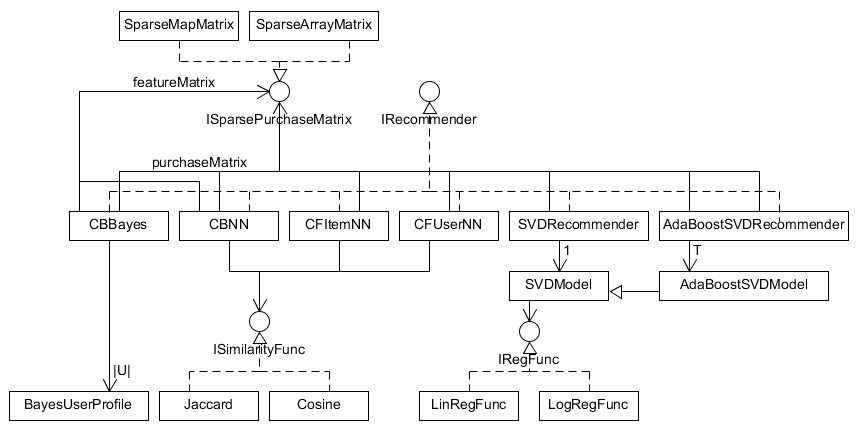
\includegraphics[width=1\textwidth]{figures/implementation/classDiagram}
	\caption{Simplified class diagram of the recommendation architecture.}
	\textit{}\label{fig:classDiagram}
\end{figure}

In order to retrieve data from different sources, an interface called \textit{IRecoData} is used.
The realizing classes have to implement the method \textit{getPurchases}, that retrieves the purchase matrix from an arbitrary source and passes it as a \textit{ISparseMatrix} implementation to a handler.
The method is called by any recommender class, where also the handlers are defined to process the returning purchase matrix.
Using a handler instead of a simple return value, ensures asynchronous computation, i.e. other operations can be made, during the purchase matrix is retrieved.
Figure \ref{fig:getPurchases} shows the UML notation of the \textit{IRecoData} interface and the sequence of obtaining the purchase matrix.


\begin{figure}
	\centering
	\begin{subfigure}[t]{0.6\textwidth}
		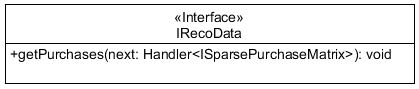
\includegraphics[width=\textwidth]{figures/implementation/IRecoDataInterface}
		\caption{Adapter interface to retrieve the purchase matrix from different sources.}
		\label{fig:irecodataInterface}
	\end{subfigure}
	\begin{subfigure}[t]{0.35\textwidth}
		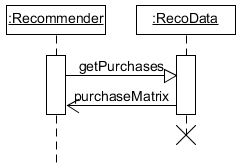
\includegraphics[width=\textwidth]{figures/implementation/getPurchasesSequence}
		\caption{Sequence of retrieving the purchase matrix from \textit{IRecoData} adapter.}
		\label{fig:getPurchasesSequence}
	\end{subfigure}
	\caption{Applied adapter pattern for different data sources.}
	\label{fig:getPurchases}
\end{figure}






%==============================================================
\chapter{Experimentation}
\label{chap:experimentation}
The described algorithms are evaluated against a real-world e-commerce dataset.
On one hand, it is aimed to compare different recommendation approaches on e-commerce data, and on the other hand, the impact of different parameters is analysed.
In the next section the data used for evaluating the algorithms is presented.
Section \ref{sec:eval} explains the used evaluation measures.
The last two sections of this chapter show the obtained results and discuss them.

\section{Data}
\label{sec:data}

\begin{figure}
	\begin{subfigure}[c]{1\textwidth}
		\centering
		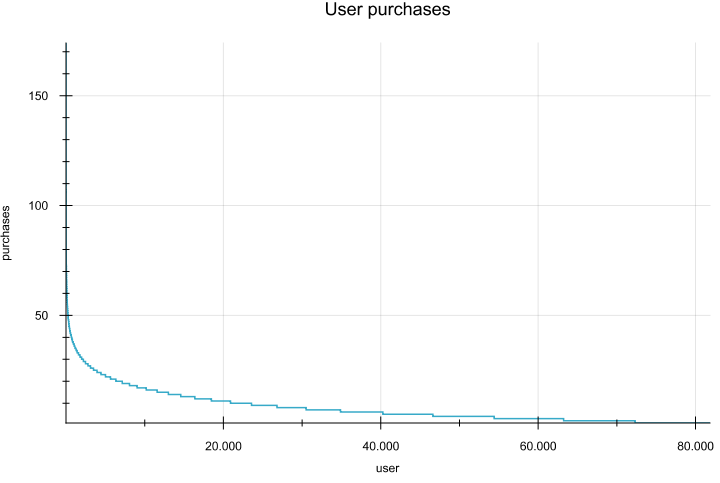
\includegraphics[width=1\textwidth]{figures/experiments/userPurchases}
		\caption{Number of purchases for every user.}
		\label{fig:userPurchases}
	\end{subfigure}
	\begin{subfigure}[c]{1\textwidth}
		\centering
		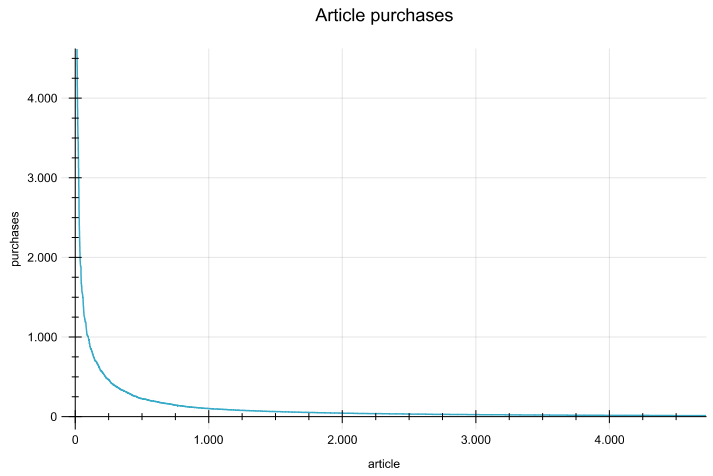
\includegraphics[width=1\textwidth]{figures/experiments/articlePurchases}
		\caption{Number of purchases for every article.}
		\label{fig:articlePurchases}
	\end{subfigure}
	\caption{Distribution of purchases.}
\end{figure}

To evaluate the different recommendation approaches, data from an online pharmacy is used.
The dataset contains purchases from 81,835 users and 14,964 articles.
Those articles contain many duplicates, because articles of the same product, but with different package sizes or different colours are considered as different articles in the database.
There is no attribute to determine real distinct articles, but the amount of duplicates was reduced by aggregating items of the same name and handle them as one item.
This reduces the number of items to 11,775.
Thus dimensions of the used purchase matrix are 81,835 \texttimes \ 11,775.
It contains 66,3731 purchases, so it is only 0.06888\% dense, there are on average 56.37 purchases per item and 8.11 purchases per user. %todo make table out of stats
Figures \ref{fig:userPurchases} and \ref{fig:articlePurchases} show the number of purchases for every user and article, respectively.
Both curves are very skewed, i.e. there are few articles and users with many purchases and many users and article with only a small amount of purchases.

%Removal of cold start users
Users, that only have purchased one item, are removed beforehand.
They cannot be evaluated, since at least one item must be left for training.
Users with no purchase are so called cold-start users and require another unpersonalized recommendation technique.
Removing those users results in a dataset of 72,318 users and 11,666 items.
In total this matrix contains 654,214 purchases, i.e. there are on average about 9.05 purchases per user and about 56.08 purchases per item.

Besides purchases there is content-based information about items.
Most items are assigned to one or more categories they belong to.
In total there are 353 different categories.
Moreover there are different kinds of texts like general information, indication, ingredients, side effects or interactions.
For evaluation purposes the texts for general information and indication are used, because they seem to be most relevant to judge the similarity of medicine.
Within the general information texts there are in total 44,755 words, the corpus of indications texts contain 21,516 words.


 \section{Evaluation}
\label{sec:eval}
The recommendation systems are evaluated using 80 percent of the data as training set to build the model and 20 percent as test set.
The test set is built by iterating user- and item-wise over purchases and adding every 5\textsuperscript{th} purchase to the test set and removing it from the training set.
This ensures, that the test purchases are equally distributed over all users.
The training set then consists of 523,371 and the test set of 130,843 instances.

An unpersonalized recommendation approach called \textit{MostPop} is used as a baseline for evaluation.
It always recommends those items to a user, that are purchased most often.

Evaluation is measured in terms of the mean average precision (MAP), a common measure in information retrieval.
It is a measure for evaluating ranked lists, since it measures precision and incorporates the ranks of true positives.
It is calculated by:

\begin{equation}
	MAP_n = \frac{1}{|U|} \sum_u^{|U|} \frac{1}{|I_u|}\sum_i^{|I_u|} Precision(i)
\end{equation}

Here $U$ is the set of users, who got recommendations in the evaluation process, and $I_u$ is the list of items, that is recommended to user $u$.
$Precision(i)$ denotes the precision of the recommended list up to position $i$, i.e. the number of correct recommendations within list elements $1$ to $i$ divided by $i$.
So it is the mean of precisions measured at every position of the list of recommendations averaged over all users, who got recommendations.
All experiments are performed calculating a ranked list of ten recommendations.
Larger lists would increase performance, because more items would participate in the evaluation and could increase the precisions.
But in an online-shop a list of more than ten recommended items would not be useful to the user, since the recommended items are not actively requested by the user, but only shown besides the user browses the shop. 


\section{Results}
\label{sec:results}
The unpersonalized approach \textit{MostPop} receives a MAP of 0.0499
The developed personalized recommendation systems are supposed to being able to outperform this approach.
%todo explain why unpersonalized recommendation performs that well

\subsection{Content-based recommendation}
The content-based naive Bayes recommender in algorithm \ref{alg:CBBayes} is applied to category information about articles.
It results in a MAP of 0.00306.
The nearest-neighbour algorithm using content-based features (algorithm \ref{alg:CBNN}) is also applied to categories, the general information and indication texts.
The texts are represented in different ways, i.e. either in binary, bag-of-words or tf-idf representation.
In all cases the cosine similarity is applied.
In the cases of category data and binary text representation also Jaccard similarity was applied. 
Results are shown in table \ref{tab:CBNN}.
It can be seen, that for binary data Jaccard similarity performs slightly better than cosine similarity as it is also the case for the memory-based collaborative filtering algorithms.
For both kind of texts, the general information and the indication, the tf-idf representation achieves best results.
With all tested content-based features the content-based recommenders both perform much worse than the unpersonalized recommender.

\begin{table}
	\begin{tabular}{|c||c|c|}
		\hline
		\textbf{Dataset}&\textbf{Jaccard}&\textbf{Cosine}\\ \hline
		categories&0.00507&0.00508\\ \hline
		indication (binary)&0.00573&0.00477\\ \hline	
		indication (bag-of-words)&-&0.00756\\ \hline	
		indication (td-idf)&-&0.00857\\ \hline	
		general information (binary)&0.01231&0.01213\\ \hline	
		general information (bag-of-words)&-&0.00804\\ \hline	
		general information (tf-idf)&-&0.01595\\ \hline	
	\end{tabular}
	\caption{Results for \textit{CBNN} applied to different content-based information and different similarity functions.}	
	\label{tab:CBNN}
\end{table}

\subsection{Memory-based collaborative filtering}
% How does CFItemNN perform with Jaccard and Cosine?
The memory-based collaborative filtering approaches are evaluated using either the Jaccard coefficient or cosine similarity.
The item-item approach (algorithm \ref{alg:CFItemNN}) will further be denoted \textit{CFItemNN}, while \textit{CFUserNN} refers to the user-user approach.

\begin{figure}
	\centering
	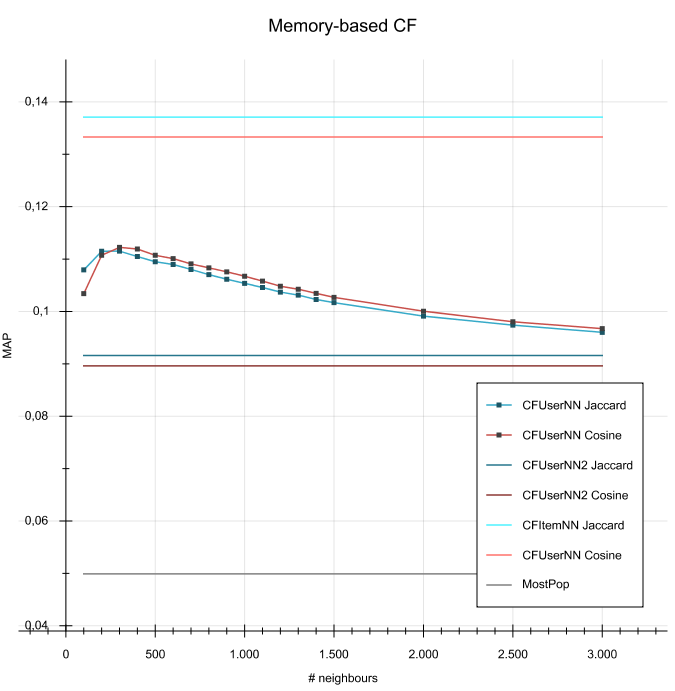
\includegraphics[width=1\textwidth]{figures/experiments/MemoryBasedCF}
	\caption{Results for \textit{CFUserNN} over different numbers of nearest neighbours (lines in the middle, with square markers), \textit{CFUserNN2} (darker lines below) and \textit{CFItemNN} (brighter lines above). Gray line at the bottom marks the unpersonalized \textit{MostPop} algorithm.}
	\label{fig:memBasedCF}
\end{figure}

The performance of \textit{CFUserNN} was measured over different neighbourhood sizes, see figure \ref{fig:memBasedCF}.
For lower neighbourhood sizes Jaccard similarity outperforms cosine similarity.
From 300 and higher number of neighbours, cosine similarity works slightly better.
The best number of nearest neighbours to be investigated to calculate the recommendation are 300.
Up to this point performance of the algorithm increases, but it decreases for larger neighbourhood sizes.
Too few neighbours are not able to suggest enough possible recommendations and recommendations are not that confident as if voted for by more neighbours.
Too many neighbours on the other hand produce fuzzy recommendations, because the neighbours may not be close enough to the current user.
MAP for more users converges to the approach of recommending the most purchased items, because \textit{MostPop} and \textit{CFUserNN} result in the same algorithm, if all users are considered as neighbours.
Algorithm \ref{alg:CFUserNN2} is also evaluated and produces a MAP of 0.0916 with Jaccard similarity and a MAP of 0.0897 with cosine similarity.
So results are worse than the observed ones from algorithm \ref{alg:CFUserNN}.
%TODO investigate size of recommendation lists...
%todo take similarity into account, use them as weights somehow

\textit{CFItemNN} performs better than the \textit{CFUserNN} resulting in a MAP of 0.1371 using Jaccard similarity and 0.1333 using cosine similarity.

\subsection{Model-based collaborative filtering}
% svd approaches

\begin{figure}
	\centering
	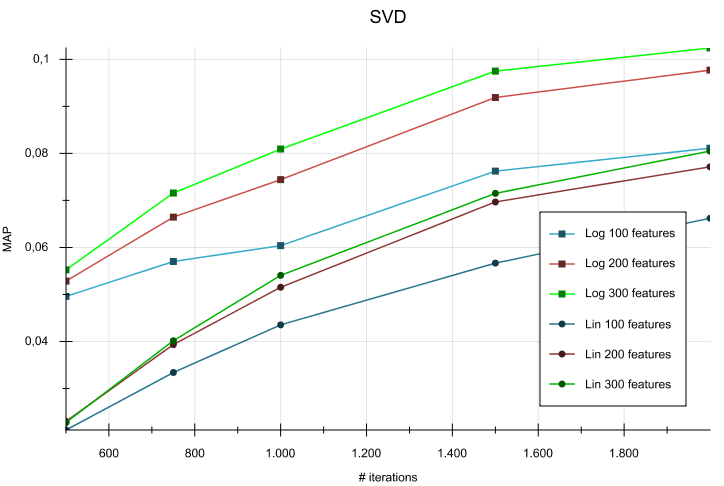
\includegraphics[width=1\textwidth]{figures/experiments/SVDIterations}
	\caption{MAPs of the SVD approaches over number of training iterations for different number of features using either traditional linear regression or the presented logistic regression formula.}
	\label{fig:SVDIterations}
\end{figure}
%todo add some iteration until curves are obviously flater

The matrix factorization approaches \textit{LogRegSVD} (see algorithms \ref{alg:LogRegSVDTraining} and \ref{alg:LogRegSVDRecommendation}) and the traditional approach using linear regression are investigated for the impact of different parameters.
All models are trained using a learning rate $\alpha$ of $0.001$, a regularization factor $\lambda$ of $0.01$ and a negative weight $w_n$ for negative instances of $0.5$, if not stated differently.
User and item features $p_u$ and $q_i$ are initialized using a Gaussian random distribution with mean 0 and a standard deviation of $0.1$.
First the number of features and iterations are investigated, to see how many features and iterations are needed to reach sufficient recommendation results.
Figure \ref{fig:SVDIterations} shows the MAP for different number of features over the number of iterations during training.
There it can be seen, that the MAP increases with the number of iterations regardless of how many features or which matrix factorization technique is used.
This is because more iterations result in a better trained model, because the feature vectors are updated more often.
\textit{LogRegSVD} outperforms the traditional SVD algorithm for every number of features and iterations.
Moreover the MAP increases, when more features are used.
The more features are used, when factorizing the purchase matrix, the more information can be preserved, similar to an ordinary singular value decomposition.
The Frobenius norm of the reduced matrix is closer to the Frobenius norm of the original matrix the greater the rank of the reduced matrix is.
Removing more features in the decomposition results in a worse approximation, but on the other hand preserves more memory and runtime.

\begin{figure}
	\centering
	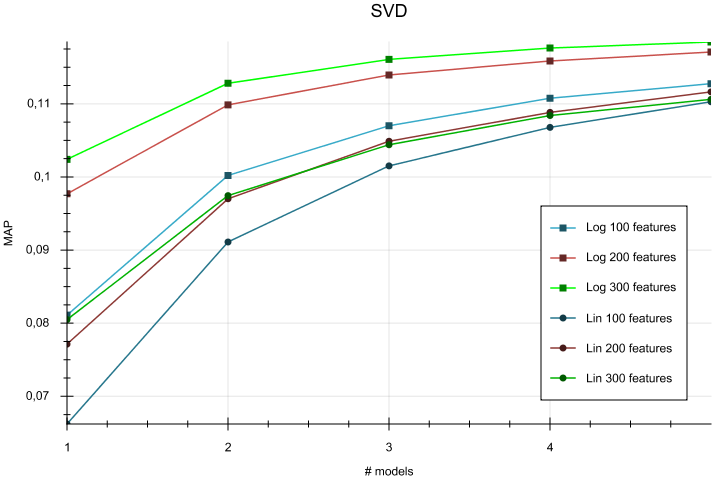
\includegraphics[width=1\textwidth]{figures/experiments/SVDModels}
	\caption{MAP for SVD approaches with AdaBoost over different number of models for different numbers of features trained in 2000 iterations.}
	\label{fig:SVDModels}
\end{figure}


\begin{figure}
	\centering
	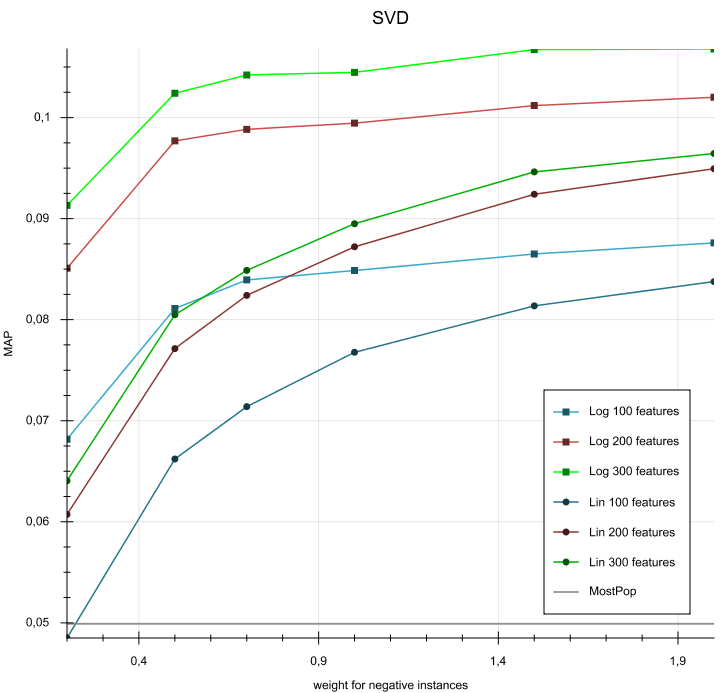
\includegraphics[width=1\textwidth]{figures/experiments/SVDWeights}
	\caption{MAP for SVD approaches over different weights for negative instances for different number of features. The models are trained with 2000 iterations.}
	\label{fig:SVDWeights}
\end{figure}

Moreover the impact of the weights of the random sampled negative feedback is investigated.
Different weights are assigned to the negative instances.
Results can be seen in figure \ref{fig:SVDWeights}.
The MAP increases for higher weights for the negative instances.
So in fact using different weights for negative instances does not bring any improvement.
Probably this results from the random sampling 
of negative instances: the negative instances are randomly sampled from the training set in every iteration, i.e. there probably is a different sample in every iteration.
So a negative instance has a much smaller impact on the trained model than the known positive instances, anyway.

\begin{figure}
	\begin{subfigure}{0.5\textwidth}
		\centering
		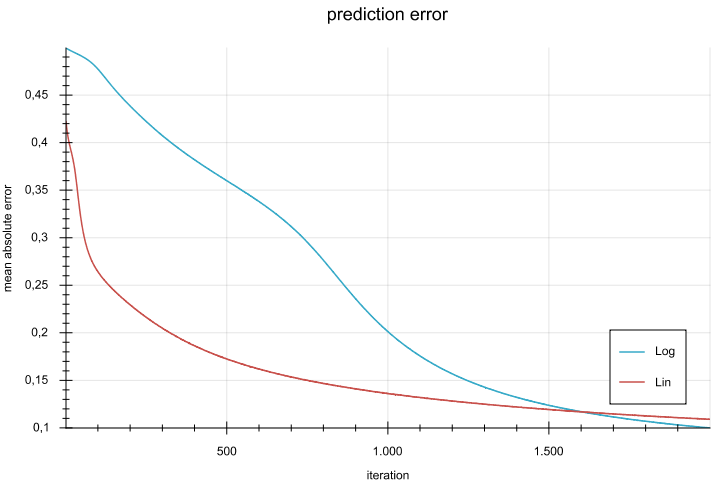
\includegraphics[width=1\textwidth]{figures/experiments/errorsLogLin43}
		\caption{Mean of absolute errors of all training instances over iterations.}
		\label{fig:errorsLogLin43}
	\end{subfigure}
	\begin{subfigure}{0.5\textwidth}
		\centering
		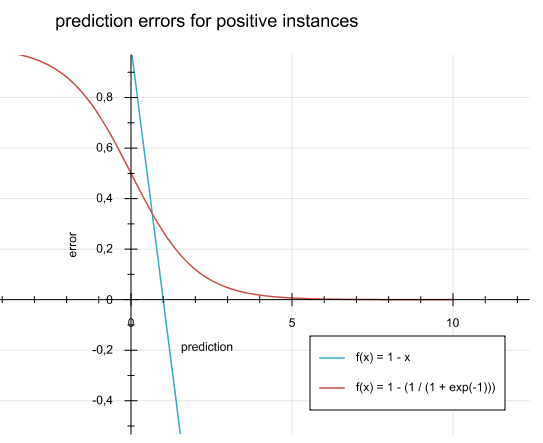
\includegraphics[width=1\textwidth]{figures/experiments/predictionErrors}
		\caption{Errors for predicted values for positive instances with linear and logistic regression function.}
		\label{fig:predictionErrors}
	\end{subfigure}
	\caption{Prediction errors for linear and logistic regression functions.}
	\label{fig:errors}
\end{figure}

The differences between the traditional matrix factorization algorithm and \textit{LogRegSVD} was further analysed by comparing the error curves they produce during the training process.
The error curves for a model with 300 features and 2000 iterations is shown in figure \ref{fig:errorsLogLin43}.
It can be seen that the curve for the linear regression approach is steeper at the beginning, but later becomes flatter than the error curve of \textit{LogRegSVD}.
The different behaviours result from the different objective functions and the impact of $p_u^Tq_i$ to it.
Figure \ref{fig:predictionErrors} shows the errors produced by linear and logistic regression for different predicted values $p_u^Tq_i$ for an positive instance.
The initial $p_u^Tq_i$ are close to zero, so the initial errors for the linear regression function are close to 1 for positive instances, while they are about 0.5 for the logistic regression function.
So at the beginning the feature updates are larger for linear regression, what results in the steeper error curve.
For linear regression the error gets zero, if $p_u^Tq_i = 1$.
For the logistic regression function in contrast the error converges to zero for $p_u^Tq_i = \infty$, while it still is $1 - \frac{1}{1 + \exp(-1)} \approx 0.27$ for $p_u^Tq_i = 1$.
So in the case of logistic regression more updates are needed to achieve good predictive results.
Nevertheless the MAP when using the models for recommendation is better for the logistic regression than for the linear regression approach.
So even if the prediction error is larger, the relation of prediction to actual user interest seems to be better than for the linear regression case.
This may result from the impact of negative instances to the training process.
While for linear regression the negative instances (i.e. $r_{ui} = 0$) push the model towards the initial state of $p_u^Tq_i \approx 0$ and cause small updates at the start of training, in the case of logistic regression, updates for negative instances actively update the feature vectors into the other direction, such that $p_u^Tq_i$ even may get negative.

\subsection{AdaBoost}
To evaluate the performance of the implemented AdaBoost approach (algorithm \ref{alg:AdaBoostLogRegSVDTraining}) the MAPs are compared for different numbers of models.
Using only one model refers to the normal SVD algorithm without boosting.
The results are shown in figure \ref{fig:SVDModels}.
As expected the MAP gets better, if more models are used.
Especially between one and two models there is a large improvement in the \textit{LogRegSVD} algorithm.
Here for 100 features the MAP increases about 23\%, for 200 features about 12\% and for 300 features about 10\%.
So already after evaluating the first model, the instance weights could be adjusted, such that instances, that are hard to predict get a better result. 
Furthermore the figure shows, that the performance difference between models with different number of features gets smaller for higher numbers of models, especially for the linear regression based SVD approach.
There the model trained with 200 features even gets better than the model with 300 features.
The differences are quite small, so this may result from the random sampling of negative instances, such that for one model a sample was generated, that produces better results, than in the other model.

\begin{figure}
	\begin{subfigure}[c]{0.5\textwidth}
		\centering
		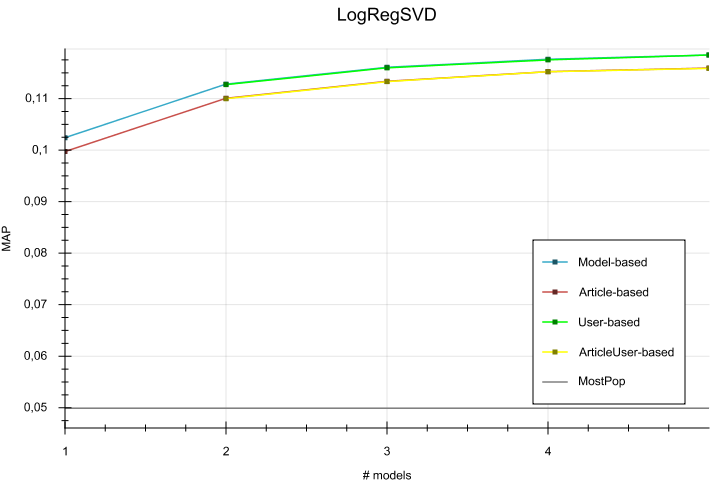
\includegraphics[width=1\textwidth]{figures/experiments/LogRegSVDPredictionsOModels}
		\caption{\textit{LogRegSVD} models}
		\label{fig:LogRegSVDPredictionsOModels}
	\end{subfigure}
	\begin{subfigure}[c]{0.5\textwidth}
		\centering
		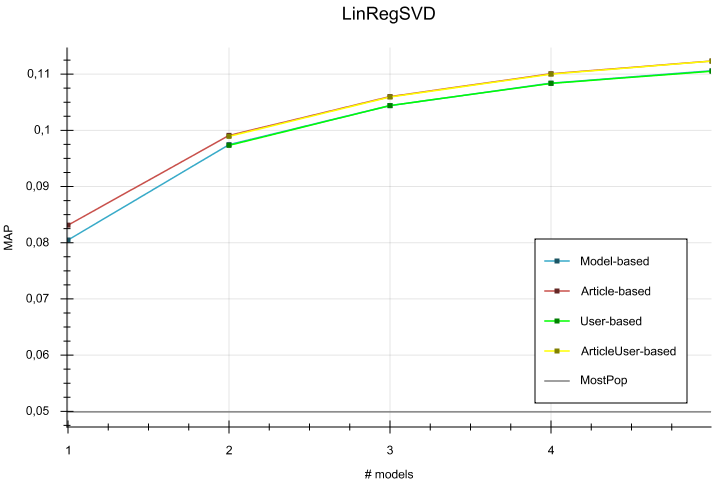
\includegraphics[width=1\textwidth]{figures/experiments/LinRegSVDPredictionsOModels}
		\caption{\textit{LinRegSVD} models}
		\label{fig:LinRegSVDPredictionsOModels}
	\end{subfigure}
	\caption{MAP of different prediction rules over the number models trained with 2000 iterations and 300 features.}
	\label{fig:SVDPredictionOModels}
\end{figure}

The presented prediction rules for the SVD and AdaBoost models are compared to each other over different numbers models as shown in figure \ref{fig:SVDPredictionOModels}. %TODO insert plots over models and explain
For the logistic regression approach none of the models can outperform the traditional prediction rule using the model error as weights.
The user-based weighting performs similar, but is slightly worse.
For the liner regression approach in contrast, the article-based and the combination of article- and user-based predictions outperform the other predictions rules.
Further plots to show the impact of the prediction rules over different numbers of features and iterations can be found in appendix \ref{app:predRulesExperiments}.



%todo add summary/comparison (as table) of best performers for every algorithm, how much better is it than baseline (in percent)?

\subsection{Error correlation of different algorithms}
To find out whether hybridizations of these techniques might be able to improve recommendation performance, the resulting lists of recommendations are investigated for correlation.
A hybrid recommender is only useful, if the component recommenders produce different results, such that they are able to complement each other.
To analyse, whether two algorithms are able to complement each other, the true positives of both recommenders are taken into account.
The amount of correct recommendations are measured, that have been recommended by both, only by one or only by the other recommender.
Only if there are many recommendations, that are only recommended by the first and many, that are only recommended by the second recommender, those recommenders might be able to be combined to a more effective hybrid recommender system.
So the recommendations of different pairs of recommenders are analysed.
Table \ref{tab:correlation} shows the amount of items, that were recommended by either both recommenders, only the first one, only the second one or by none them.
First it can be seen, that none of the content-based recommenders is able to enhance recommendation, when combined with another approach.
In the performed experiments a content-based recommender reaches at most 2.42\% of recommendation, that would not have been recommended by another collaborative filtering recommender.
The most promising combination of recommenders seems to be the user-user and the boosted logistic regression based recommender.
\textit{CFUserNN} is able to provide 11.32\% and \textit{LogRegSVD} 8.88\% of recommendation that have not been found by the other one, though both are collaborative filtering approaches.
This might come from serendipitous recommendations made by the user-user approach.
While the other collaborative filtering approach tend to provide items, that are similar to those the current user already purchased, \textit{CFUserNN} might also find items, that are dissimilar, but are bought by some similar users.

\begin{table}
	\begin{tabular}{|c|c||p{1.2cm}|p{1.2cm}|p{1.2cm}|p{1.2cm}|}
		\hline
		\textbf{R. 1}&\textbf{R. 2}&\textbf{both}&\textbf{only R. 1}&\textbf{only R. 2}&\textbf{none}\\ \hline
		\textit{CFItemNN}&\textit{CBNN (Categories)}&400 (0.31\%)&25446 (19.45\%)&1185 (0.91\%)&103812 (79.34\%)\\ \hline
		\textit{CFItemNN}&\textit{CBNN (Categories)}&550 (0.42\%)&28602 (21.86\%)&1035 (0.79\%)&100656 (76.93\%) \\ \hline
		\textit{CFUserNN}&\textit{CBNN (text)}&1047 (0.80\%)&24789 (18.95\%)&3165 (2.42\%)&101833 (77.83\%) \\ \hline
		\textit{CFIemNN}&\textit{CBNN (text)}&1713 (1.31\%)&27971 (21.38\%)&2499 (1.91\%)&98660 (75.4\%) \\ \hline
		\textit{CFItemNN}&\textit{CFUserNN}&20965 (16.02\%)&8719 (6.66\%)&4882 (3.73\%)&96277 (73.58\%) \\ \hline
		\textit{CFItemNN}&\textit{LogRegSVD}&16795 (12.84\%)&12889 (9.85\%)&5857 (4.48\%)&95302 (72.84\%) \\ \hline
		\textit{CFUserNN}&\textit{LogRegSVD}&11035 (8.43\%)&14811 (11.32\%)&11617 (8.88\%)&93380 (71.37\%) \\ \hline
		 \textit{CBNN}&\textit{LogRegSVD}&1769 (1.35\%)&2443 (1.87\%)&20883 (15.96\%)&105748 (80.82\%)\\ \hline
	\end{tabular}
	\caption{Common recommendations for different pairs of recommenders. \textit{CFUserNN} were applied for 300 neighbours. \textit{CBNN} (text) refers to algorithm \ref{alg:CBNN} using text with general information represented. For \textit{LogRegSVD} a boosted version with 5 models, 300 features trained in 2000 iteration is used. All nearest neighbour algorithms are applied with Jaccard similarity, except for \textit{CBNN} with text. There cosine similarity is used.}
\label{tab:correlation}
\end{table}

\subsection{Candidate threshold}
To speed up recommendation a cascade hybrid system was implemented.
Figure \ref{fig:articlePurchases} shows the number of purchases for every article.
It can be seen, that there are few items with many purchases, and that most items just have few purchases.
The items with many purchases generally have a higher probability of being purchased, i.e. being a correct recommendation.
In order to avoid to iterate through the full list of items to make a recommendation, only those items are taken into account, that were purchased at least $c$ times.
$c$ will further be denoted as candidate threshold, since it delimits the number of candidates for recommendations.
This approach can be viewed as a cascade hybrid between the \textit{MostPop} and any other recommendation approach.
It was applied to different recommendation systems to see, whether it diminishes or even improves recommendation performance.
Results for different recommendation approaches can be seen in figure \ref{fig:candidates}.
For \textit{CFItemNN} slight improvements can be seen up to a threshold of 10.
Higher thresholds decrease the MAP again.
Even the best performing threshold only reaches an improvement of about 1.5\% in contrast to a threshold of 1, i.e. using all items as possible recommendation candidates.
\textit{LogRegSVD} performs worse the higher the candidate threshold gets.
The number of purchases of an item effects the training of the model anyway, so reducing the set of candidates with respect to their number of purchases cannot improve the SVD-based approaches.
For \text{CBNN}, applied on general information text represented as tf-idf values, a smaller set of candidates marginally increases the MAP up to about 400 candidates.
Then the MAP stagnates for higher thresholds.
This approach still performs significantly worse than the \textit{MostPop} approach.
\textit{CFUserNN} already determines the most purchased items of a user's neighbours.
So this hybrid was not applied to \textit{CFUserNN}.
Moreover the set of recommended items is not guaranteed to be large enough anyway, without further restricting the candidates for recommendations.
Runtime improvements also cannot be achieved here, because the main part of the algorithm iterates over the set of users instead of items.


\begin{figure}
	\begin{subfigure}[c]{0.5\textwidth}
		\centering
		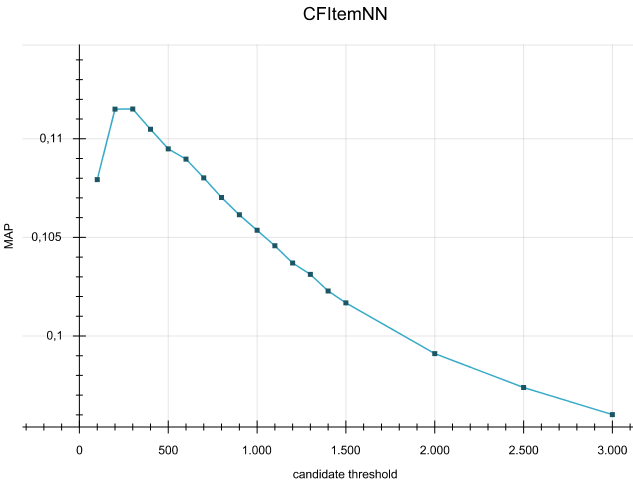
\includegraphics[width=1\textwidth]{figures/experiments/CFItemNNCandidates}
		\caption{MAP of \textit{CFItemNN} over different candidate thresholds.}
		\label{fig:CFItemNNCandidates}
	\end{subfigure}
	\begin{subfigure}[c]{0.5\textwidth}
		\centering
		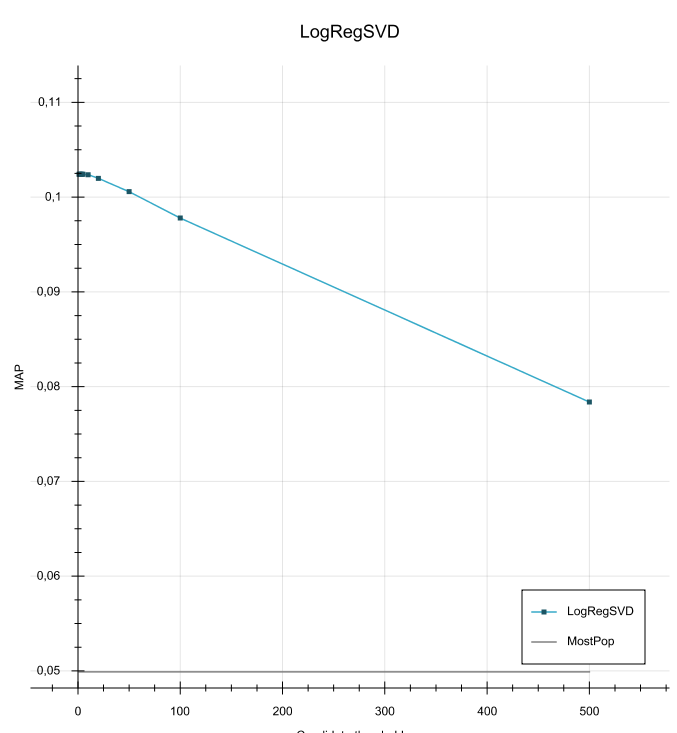
\includegraphics[width=1\textwidth]{figures/experiments/LogRegSVDCandidates}
		\caption{MAP of \textit{LogRegSVD} over different candidate thresholds.}
		\label{fig:LogRegSVDCandidates}
	\end{subfigure}
	\begin{subfigure}[c]{0.5\textwidth}
		\centering
		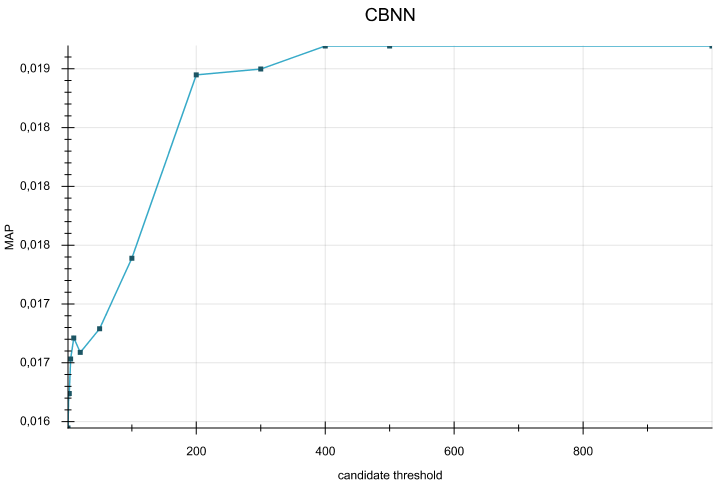
\includegraphics[width=1\textwidth]{figures/experiments/CBNNCandidates}
		\caption{MAP of \textit{CBNN} over different candidate thresholds.}
		\label{fig:CBNNCandidates}
	\end{subfigure}
	\caption{Impact of candidate threshold for different approaches}
	\label{fig:candidates}
\end{figure}


\section{Discussion}
\label{sec:discussion}
In the last section several experiments and their results are presented.
This sections aims to analyse the results.
The weaknesses and strengths of the basic recommendation systems in e-commerce context are pointed out.
The success of the presented \textit{LogRegSVD} algorithm is discussed.
Moreover the performance of the AdaBoost approach and the applied prediction rules are summarized.

\subsection{Single recommendation systems}
\label{sec:discSingleRecommendationSystems}
% Memory-based: CFItem works better
The experiments performed for the memory-based collaborative filtering approaches show, that the item-item approach performs best on the e-commerce dataset.
\textit{CFItemNN} probably works better, because the similarity of items are more confident than the similarity of users, since the item vectors are larger than the user vectors.
For the user-user similarity approaches it was shown, that algorithm \ref{alg:CFUserNN} outperforms algorithm \ref{alg:CFUserNN2}, though the second algorithm requires much more runtime.
The recommendations of algorithm \ref{alg:CFUserNN2} might be too fuzzy, because all users' preferences are taken account instead of only those users' purchases, that are similar to the current user.
For both algorithm \ref{alg:CFItemNN} and \ref{alg:CFUserNN} it was shown, that Jaccard similarity results in a slightly better MAP than cosine similarity.

%  LogRegSVD
The presented \textit{LogRegSVD} approach (algorithm \ref{alg:LogRegSVDTraining} and \ref{alg:LogRegSVDRecommendation}) is much faster in making recommendation, but performs worse than the memory-based approaches.
This might be due to the fact, that information gets lost when factorizing the purchase matrix into smaller feature vectors.
Using larger matrices might improve the results as figure \ref{fig:SVDIterations} indicates, but using larger feature vectors does not only slow down training of the model, but also slows down the recommendation process, because vector multiplication has to be performed on larger feature vectors.

% contentbased are even much worse than mostpop, because too similar
The content-based approaches in algorithms \ref{alg:CBBayes} and \ref{alg:CBNN} perform much worse than the collaborative filtering approaches.
They are even worse than the unpersonalized approach of recommending the most purchased item.
This results from the nature of e-commerce data.
The dataset contains duplicate items, that only differ in brand, size of package, colour or the like.
So items, that are recommended by a content-based recommender, are probably too similar to the items the current user already purchased, since he probably will not buy products, that are almost equal to those, he already bought.


\subsection{AdaBoost}
\label{sec:discAdaBoost}
% Outperfroms CFUserNN, but worse than CFItemNN
AdaBoost using 5 models achieves an improvement in the MAP of about 15\% as compared with a single \textit{LogRegSVD} model.
So focussing on instances with a high recommendation error in the training process increases the recommendation performance.
Probably the instances with higher errors are those, that have only few entries in the purchase matrix, such that AdaBoost achieves a more balanced training process between instances of different numbers of purchases.
The boosted \textit{LogRegSVD} outperforms the user-user approach, but still performs worse than the memory-based item-item approach, but the recommendation process is much faster and less memory intensive, because it does not require the full purchase matrix.
%todo see whether instance error correlate with number of purchases

\subsection{Prediction rules}
\label{sec:discPredRules}
% prediction rules were not able to improve performance, if model is sufficiently trained
The alternative prediction rules suggested for multiple or single \textit{LogRegSVD} models were not able to improve the MAP.
It only outperformed the traditional prediction rules for single \textit{LogRegSVD} models, that have not been sufficiently trained, i.e. models that have been trained with to few number of iterations.
In those cases the article based prediction, see equation \ref{eq:articleErrorPrediction}, is able to outperform the traditional prediction approach.
%TODO update after plot over model is added

\subsection{Hybrid recommendation systems}
\label{sec:discHybrid}
The experiments performed to investigate error correlations of the single hybrids showed, that combinations between a content-based and a collaborative filtering approach cannot enhance recommendation performance, since there is only a very small amount of maximal 2.42\% of recommendations, that can be found a content-based recommender, but not by another collaborative filtering one.
The combinations between different collaborative filtering approaches make more diverse errors, especially \textit{CFUserNN} and the boosted version of \textit{LogRegSVD}.
So the only hybrid recommenders, that may be able to improve recommendation results, are combinations between collaborative filtering  approaches.
Combining two memory-based approaches probably would require a lot more runtime for making recommendations, because there are two models, that have to process the whole purchase matrix.
But hybrids between a memory-based and a model-based recommender may be feasible, if the memory-based approach can be incorporated in the training process of the model-based recommender, such that actual recommendation computation will not significantly be slowed down by processing the whole purchase matrix. %todo reference to corresponding hybrid if I add that chapter

The hybrid recommender using the unpersonalized \textit{MostPop} approach and any other personalized recommendation showed small improvements over the single unpersonalized ones.
This is due to the removal of items that are rarely purchased and therefore have a lower probability to be purchased.
The improvements only occur up to specific thresholds, otherwise relevant items are removed by the \textit{MostPop} recommender as well.
Moreover it was shown that it slightly decreases recommendation computation time, because the most purchased items can be precomputed, such that the set of items that have to be taken into account by the personalized recommender is smaller in the actual recommendation step.




%==============================================================
\chapter{Conclusion and Future work}
\label{chap:conclusionAndFutureWork}
In this work several common recommendation techniques are implemented and applied to an e-commerce dataset.
In detail the recommenders are a user-user and an item-item memory-based collaborative approach, a new matrix factorization approach, adapting a common SVD-based approach to binary data called \textit{LogRegSVD}, and content-based recommendation techniques.
The recommenders are evaluated using the mean average precision when trained on a training set consisting of 80\% of the data, and a test set consisting of the remaining 20\%.
It was shown, that the item-item approach performs best on this dataset, but conflicts with the requirement of online shops to provide immediate recommendations.
This could be solved by precomputing and storing the similarities between every user and item pairs, which would require a large amount of memory.
User-User approaches reach a MAP of at leas twice as good as the unpersonalized baseline predictor.
The \textit{LogRegSVD} approach was able to outperform the user-user approach, both in terms of MAP and computation time.
Results are still worse than those provided by the item-item approach, but recommendation can be made faster, because only a pretrained model needs to be computed instead of the full matrix of all purchases.
The results of this approach are tried to be enhanced by applying AdaBoost to it, a meta algorithm to improve results of weak classifiers.
Results can be enhanced by 16\% to 39\%, depending on the number of trained latent features.
Moreover alternative prediction rules are suggested, that incorporate different types of errors to express confidence of prediction.
These rules did not show any remarkable improvements in recommendation process.
The content-based recommendation systems showed results, that were much worse than those provided by the unpersonalized recommender.
This is due to duplicate item in e-commerce datasets.
The user gets recommendations of items, that are almost equal to those, he already purchased, but only differ in brand, size or colour.

Moreover the errors of the evaluated recommenders are analysed for correlation to find candidates for possible hybridization of different recommenders.
The only candidates for hybridization are combinations of the presented collaborative filtering approaches, especially between \textit{CFUserNN} and boosted \textit{LogRegSVD}.
Combinations between the unpersonalized and the other approaches were implemented as a cascade hybrid recommendation system.
This approaches removes rarely purchased items from the set before finding recommendations, such that the personalized recommenders have to process a smaller set of items.
This hybridization achieves slight improvements in computation time and MAP for the item-item based collaborative filtering approach up to a specific threshold.
For the content-based recommenders there is an improvement of the MAP as well, but it still performs much worse than the unpersonalized recommender.

Tasks for future work are on one hand investigations of possible hybrid systems, especially consisting of the presented \textit{LogRegSVD} and the user-user approach.
The challenge here is to find a hybridization technique, that does not diminish the advantages of the model-based recommenders concerning a shorter runtime for recommendations.
Techniques need to be investigated that incorporate the user-user algorithm into the training process of the \textit{LogRegSVD} models.

Further experiments for the boosted \textit{LogRegSVD} model can be made by trying to apply the user and article errors to the training process instead of prediction process.
Updating the instance weights may than be performed with respect to the errors of users and articles instead of instance or whole model errors.

Another problem of recommendation in e-commerce systems still is the lack of negative feedback.
Recommendations are constant as long as the user does not make further purchases, because they cannot be marked as not needed by the user.
A possible solution can be to take context or time into account.
Context may refer to the current or recent article views or queries of the user, such that the system is able to react on current needs.
Taking time into account means on one hand, that it could be made use of purchase sequences.
On the other hand recommended items, that have not been purchased or even clicked in some time will be penalized during the recommendation process or are interpreted as not interesting for the user.

The problem of recommending too similar items when applying content-based recommenders can be addressed by developing a clustering technique to find equal or very similar items and then perform further experiments on the found clusters. 
This approach was already implemented by \cite{hybridCFCBClustringLi} and successfully applied to a rating dataset for movies. 



\bibliography{thesis_report}
\bibliographystyle{unsrt}

\appendix
	\chapter{Results of prediction rules}
	\label{app:predRulesExperiments}
	Here some additional plots to evaluate the performance of the prediction rules presented in section \ref{sec:predictionRules} are given.
	
	\begin{figure}[h!]
		\begin{subfigure}[c]{0.5\textwidth}
			\centering	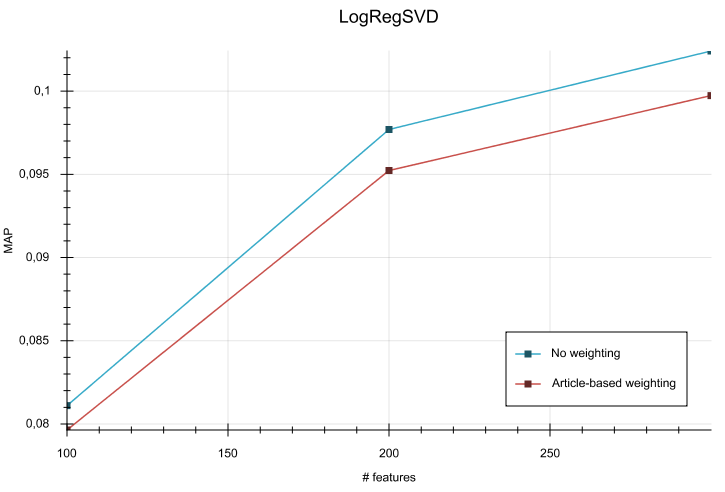
\includegraphics[width=1\textwidth]{figures/experiments/LogRegSVDPredictionOverFeatureNumSingle}
		\end{subfigure}
		\begin{subfigure}[c]{0.5\textwidth}
			\centering
			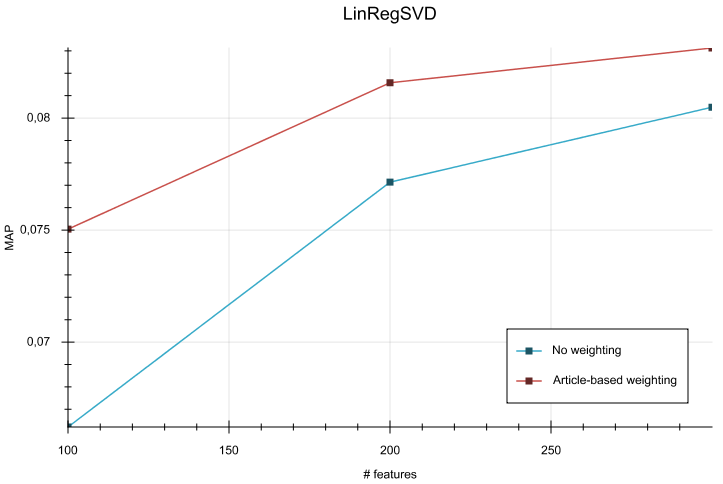
\includegraphics[width=1\textwidth]{figures/experiments/LinRegSVDPredictionsOFeaturesSingle}
		\end{subfigure}
		\caption{Different prediction rules applied to a single SVD model over number of features. Models are trained with 2000 iterations, a learning rate $\alpha$ of 0.001, a regularization factor $\lambda$ of 0.01 and a weight $w_n$ of 0.5 for negative instances. User and item features $p_u$ and $q_i$ are initialized using a Gaussian random distribution with mean zero and a standard deviation of $0.1$.}
	\end{figure}
	\begin{figure}[h!]
		\begin{subfigure}[c]{0.5\textwidth}
			\centering
			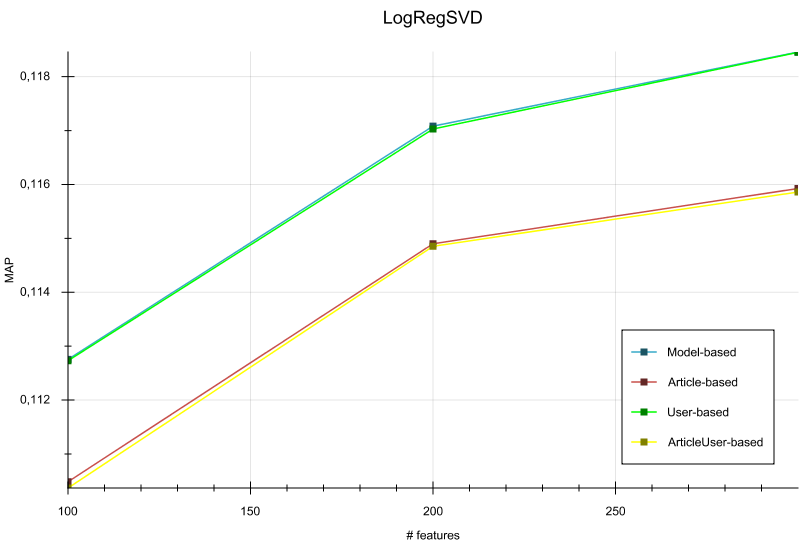
\includegraphics[width=1\textwidth]{figures/experiments/LogRegSVDPredictionOverFeatureNumBoost}
		\end{subfigure}
		\begin{subfigure}[c]{0.5\textwidth}
			\centering
			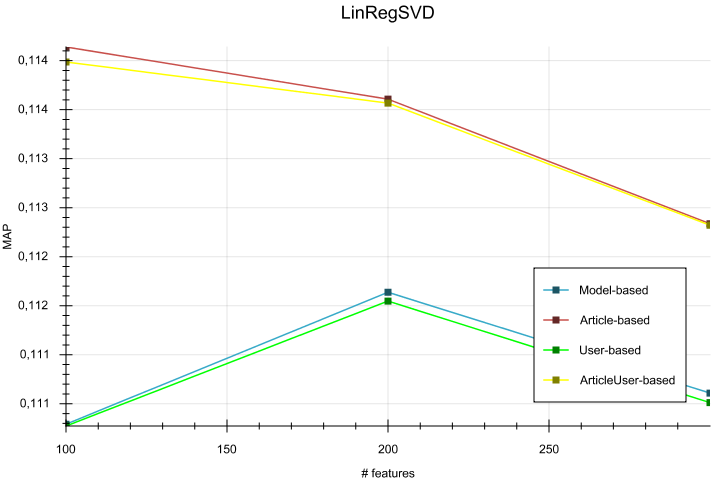
\includegraphics[width=1\textwidth]{figures/experiments/LinRegSVDPredictionsOFeaturesBoost}
		\end{subfigure}
		\caption{Different prediction rules applied to 5 boosted SVD models over number of features. Models are trained with 2000 iterations, a learning rate $\alpha$ of 0.001, a regularization factor $\lambda$ of 0.01 and a weight $w_n$ of 0.5 for negative instances. User and item features $p_u$ and $q_i$ are initialized using a Gaussian random distribution with mean zero and a standard deviation of $0.1$.}
	\end{figure}
	\begin{figure}[h!]
		\begin{subfigure}[c]{0.5\textwidth}
			\centering	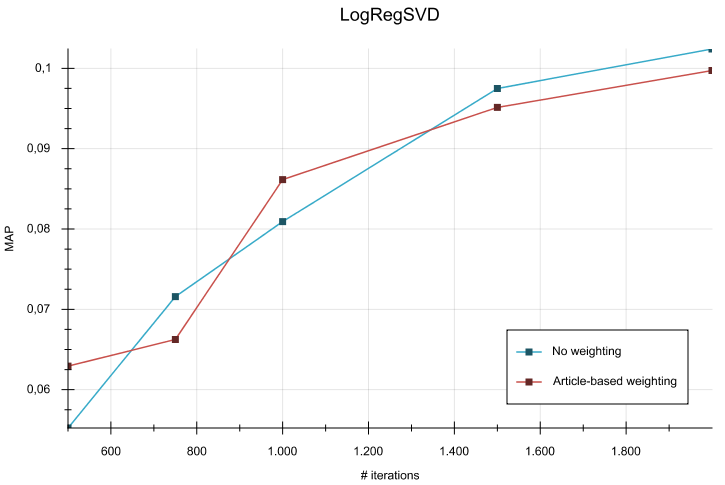
\includegraphics[width=1\textwidth]{figures/experiments/LogRegSVDPredictionOverIterationNumSingle}
		\end{subfigure}
		\begin{subfigure}[c]{0.5\textwidth}
			\centering
			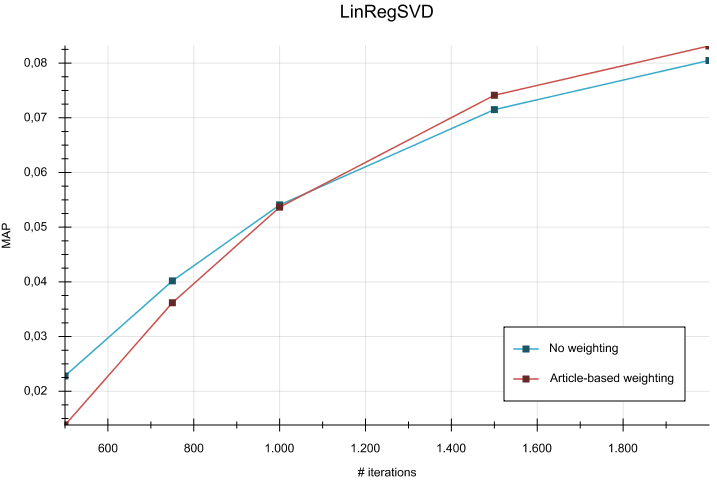
\includegraphics[width=1\textwidth]{figures/experiments/LinRegSVDPredictionsOIterationsSingle}
		\end{subfigure}
		\caption{Different prediction rules applied to a single SVD model over number of iterations. Models are trained with 300 features, a learning rate $\alpha$ of 0.001, a regularization factor $\lambda$ of 0.01 and a weight $w_n$ of 0.5 for negative instances.}
	\end{figure}
	\begin{figure}[h!]
		\begin{subfigure}[c]{0.5\textwidth}
			\centering
			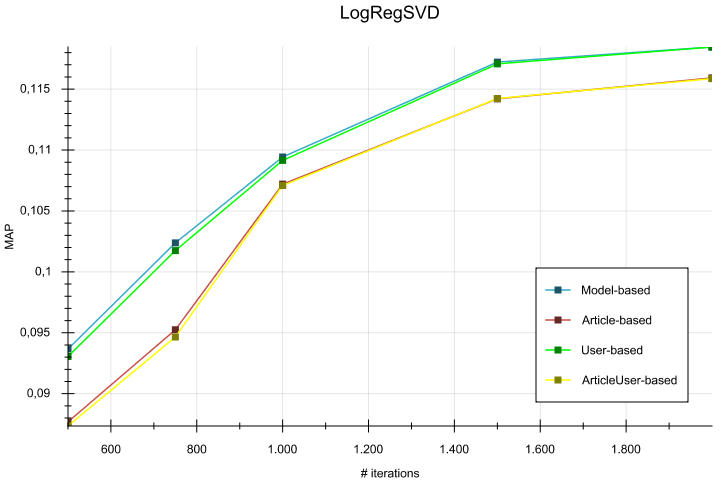
\includegraphics[width=1\textwidth]{figures/experiments/LogRegSVDPredictionOverIterationNumBoost}
		\end{subfigure}
		\begin{subfigure}[c]{0.5\textwidth}
			\centering
			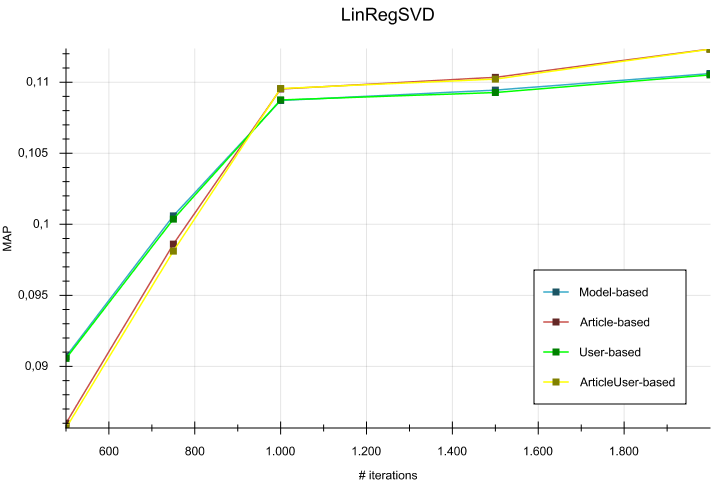
\includegraphics[width=1\textwidth]{figures/experiments/LinRegSVDPredictionsOIterationsBoost}
		\end{subfigure}
		\caption{Different prediction rules applied to 5 boosted SVD models over number of iterations. Models are trained with 300 features, a learning rate $\alpha$ of 0.001, a regularization factor $\lambda$ of 0.01 and a weight $w_n$ of 0.5 for negative instances.}
	\end{figure}

\end{document}

